%#! platex main.tex
\documentclass[a4paper,12pt]{jreport}
\usepackage{jgraduate}          % 卒論・修論用スタイル

%% 索引作成
%\usepackage{makeidx}
% dvipdfmxを使用しない場合はオプションを変更すること
\usepackage[dvipdfmx]{graphicx}
% 数字付きリストでラベルを使う
\usepackage{enumerate}
% 数学記号など
\usepackage{amsmath}
\usepackage{amssymb}
\usepackage{amsthm}
% URLをいい感じにする
\usepackage{url}
\usepackage{cite}
% キャプション
\usepackage{subcaption}

%------------------------------
% 余白設定
%------------------------------
\usepackage[left=27mm,right=27mm,top=45mm,bottom=45mm,%
 headheight=5mm,headsep=10mm,%
 footskip=12mm%
 ]{geometry}

%------------------------------
% hyperref
%  日本語の文字コード設定が分からない人はコメントアウトすること.
%------------------------------
% PDF化したときにしおりが作成され,図表へのジャンプも可能となる.
\usepackage{atbegshi}
% Mac/Linuxの場合
%   ※Ubuntuの場合はEUC-UCS2を自分で入れないとダメ.
\AtBeginShipoutFirst{\special{pdf:tounicode EUC-UCS2}}
%% Winの場合
%\AtBeginShipoutFirst{\special{pdf:tounicode 90ms-RKSJ-UCS2}}
% 以下は共通
\usepackage[dvipdfm,a4paper,bookmarks,bookmarksnumbered,%
 hidelinks,% 目次やリンクテキストの周囲の赤枠を消す
 bookmarksopen=false,pdfstartview={FitH},%
 bookmarkstype=toc,%
 setpagesize=false,%
 pdfauthor={大平 祐大},%
% setpagesize=false,% PDFのサイズがおかしい場合はこれを有効化
 pdftitle={master_thesis}]{hyperref}

%----------------------------------------------------------------------
% 設定
%----------------------------------------------------------------------
% 目次の深さはsubsubsectionまで
\setcounter{tocdepth}{3}

% 基準となる図の幅
\newlength\figurewidth
\setlength{\figurewidth}{0.8\textwidth}
% 縦に並べた図の間の基準となるスペース
\newlength\figuresep
\setlength{\figuresep}{0.8\floatsep}

%----------------------------------------------------------------------
% 文書基本情報
%----------------------------------------------------------------------
% タイトル
\title{咀嚼音に基づく食事行動の\\センシング手法と食事行動改善に向けた\\アプリケーションの提案}

% 著者
\author{大平 祐大}

% 所属
\university{九州大学大学院}
\department{システム情報科学府}
\course{修士課程}
\major{情報理工学専攻}
% \submajor{情報理工学コース}

% 提出日(月までを書く)
\date{令和6年2月}

%% 書いている途中では以下のようにしておくと一部だけをタイプセットできる
% \includeonly{intro}

%======================================================================
% テキスト開始
%======================================================================
\begin{document}
% 表紙
\maketitle
% 表紙はページ番号を出力しない
\thispagestyle{empty}

%----------------------------------------------------------------------
% 概要
%----------------------------------------------------------------------
\begin{abstract}
    食事管理アプリケーションの登場により食品名やカロリーの自動記録が可能になっているが, 健康管理の観点では, 食べる順番, 食べる速度, 咀嚼の回数といった食べ方の情報も重要な要素である. このような食事過程のセンシングを試みる先行研究は存在するが, 独自に開発された専用デバイスの装着が必要不可欠であり, その普及には課題が残っている. そこで, 本研究ではすでに普及している市販のイヤラブルデバイスとスマートフォンのみを使用し, 食事内容と咀嚼回数の推定が可能なセンシング手法を提案する. 具体的には, 食事中に発生する音をメルスペクトログラムに変換し, 畳み込みニューラルネットワークで学習させ, 食事内容推定モデルの作成を行う. また, メルスペクトログラムの各時間軸毎の全ての周波数帯の信号強度の平均をとり, ピーク検出を行うことで咀嚼の検出を行う. 本研究では, データ収集のために, 食事中に発生する音を録音しつつ, 被験者自身が咀嚼回数をカウントできる独自のアプリケーションを開発した. データ収集実験では, 15名の被験者を対象にアプリケーションを配布し, ワイヤレスイヤホンを装着した状態で, 一品ずつ食事を行った. また, 咀嚼検出の分析のために, 実験中に被験者自身の咀嚼回数をカウントするように指示した. 16種類の食品に対して録音を行い, 合計で13422秒の音データを得られた. その結果, 収集した音データで食事内容推定モデルを学習させたところ, 検証用の音データに対して, 精度$77.5\%$で食事内容を推定できることを確認した. また, 10秒間の音データに対して被験者がカウントした咀嚼回数とピーク検出回数との間の平均絶対値誤差$MAE$を算出したところ, $MAE = 4.9$を確認することができた.
\end{abstract}

%----------------------------------------------------------------------
% 目次のページ番号は1から
\setcounter{page}{0}
% 目次
\tableofcontents

% 本文のページ番号はアラビア数字
\pagenumbering{arabic}

%======================================================================
% 本文ここから
%======================================================================

% 章ごとのファイルを読み込む
% YaTeXなら各ファイルを読み込む行でC-c gでジャンプできる
%#! platex main.tex

%======================================================================
\chapter{はじめに}
\label{cha:intro}

近年, 食事管理アプリにより, 食事の写真から食品やカロリなどの栄養素を自動で記録できるようになってきた. これらの技術は, 食事の写真から画像認識技術により, 食品を特定し, 栄養データを算出することがベースとなっている. 例えば, カロミル\footnote{健康管理アプリ、カロミルとは?|食事内容・日々の体重・運動量をアプリで簡単に記録~\url{https://www.calomeal.com/}}は, iOS・Androidアプリとして提供されており, スマートフォンのカメラで食事の写真を撮るだけで, 食事の内容を解析し, 自動で摂取栄養素を記録することができる.

一方で, 健康的な食事を行う上で, 摂取栄養素だけでなく食べる順番やスピードを意識することは非常に重要である. 日本の学校教育では, 米やパンなどといった主食と, 汁物や飲料, おかずを順序よく食べる方法「三角食べ」を推奨していた. 学術面においても, 食べる順番に重点をおいた食事指導の有効性については関西電力医学研究所の研究グループにより証明されており, 最初の5分間は食物繊維を含む食品やタンパク質や脂質を含む食品を食べ, その後, 炭水化物を含む食品を, 食物繊維を含む食品やタンパク質や脂質を含む食品と一緒に食べるよう指導すると, 体重の減量に影響を与えることを報告した\cite{yabe2019107450}. さらに, 糖尿病予防にも効果があり, 野菜から先に摂取すると, 米飯から先に摂取した場合と比較して食後の血糖値の上昇を抑えることができる\cite{tonyobyo53112}. また, 食べる速度についても, 早食いは肥満や糖尿病, 心臓に対して悪影響を及ぼすことが明らかになっている\cite{20249}\cite{beyond_willpower}. 以上の事実から, 一品ずつ集中して食べる「ばっかり食べ」や咀嚼をあまり行わない「早食い」をする子供に対して注意することは妥当であると言える.

\begin{figure}[t]
  \begin{center}
    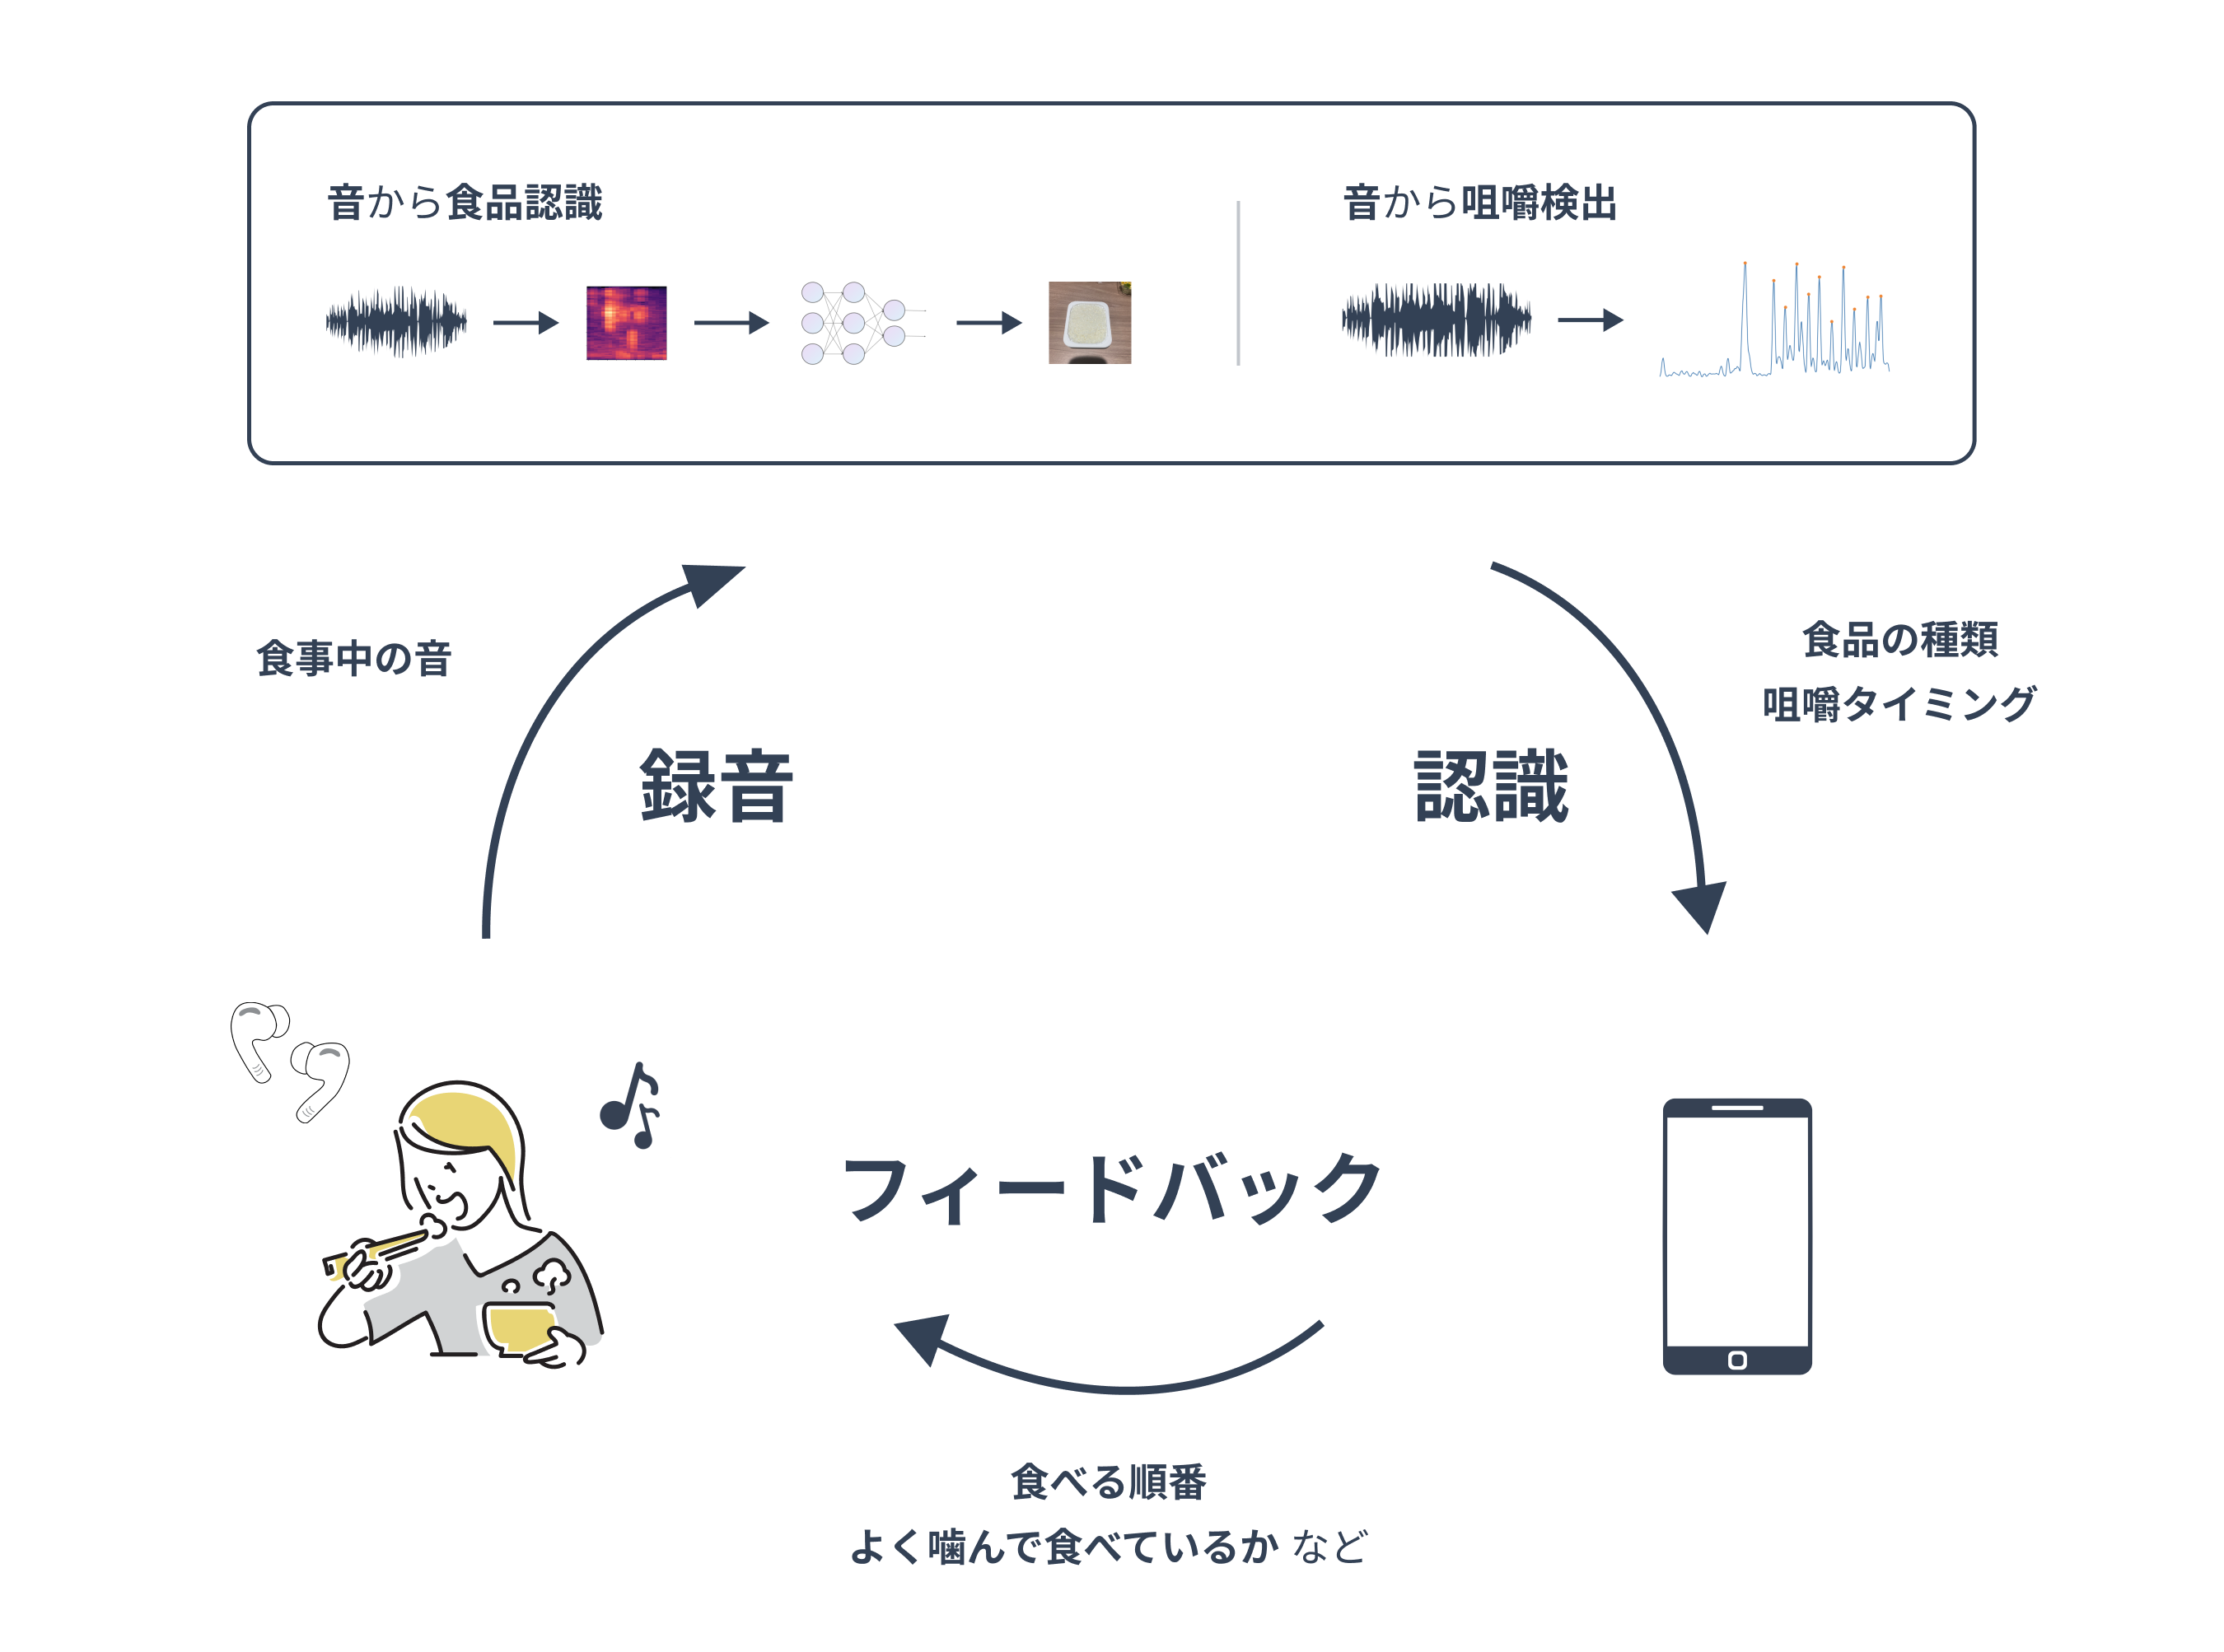
\includegraphics[clip, width=1.0\hsize]{img/system.png}
    \caption{食事中の音から食事行動をフィードバックするシステム}
    \label{fig:system}
  \end{center}
\end{figure}

食べる順番や速度などを含む食事行動の記録やフィードバックに着目した研究やプロダクトも存在する. シャープが開発したbitescan\footnote{咀嚼計「bitescan(バイトスキャン)」:シャープ~\url{https://jp.sharp/business/bitescan/}}では, 独自の耳掛け式のウェアラブルデバイスを用いて, 食事中にリアルタイムで咀嚼検出を行うことで, 咀嚼テンポや食事の時間などを記録し, フィードバックすることができる. しかし, 独自のウェアラブルデバイスが必要となるため, 普及性の観点で課題があり, そもそも咀嚼回数のみを計測しているため, 食べる順番を記録することができない. また, ウェアラブルデバイスで食事行動を撮影した一人称映像から食事内容をリアルタイムで検出する研究も存在するが, この手法も食事中にカメラで撮影し続ける必要があるため, 一般的な食事シーンで計測を行うのは受け入れ難い\cite{10.1145/3551626.3564964}.

我々の研究グループでは, 健康的な食生活を促進する行動変容支援システムとしてeat2picを提案している\cite{10.1145/3580784}. eat2picは物理世界における「食べる」行動をモニタリングし, それをデジタルな「描く」世界に反映させるナッジングシステムである. 独自の箸型センサを用いて一口ずつ何をどのくらいの速度で食べたかを自動で追跡し, 食事行動の良し悪しを絵画で表現することで, リアルタイムの視覚的フィードバックを提供している. しかし, eat2picのセンシングアプローチはカメラとIMUを搭載した専用の箸型センサを使用する必要があるため, 日常生活での利便性や社会全体への普及可能性という観点で, 課題が残っている. また, 既存のeat2picシステムは食材を噛むという動作に応じて絵を描くというインタラクションは未対応となっている. eat2picが噛む動作に対応することができれば, 絵を用いた介入によって, よく噛んで食べるといった健康的な食事行動を誘引できる可能性が広がる.

本研究では, すでに普及している市販のイヤラブルデバイスとスマートフォンのみを使用し, 食品推定と咀嚼検出が可能なセンシング手法を提案する. さらに, 本研究が提案するセンシング手法を用いた食事行動のフィードバックシステム(図\ref{fig:system})の一例として, eat2picのナッジメカニズムをベースに, 「噛む」動作に応じてデジタルな「描く」世界に反映させる「Chew-Draw」という新たなインタラクションを提案する.

本稿では, 食事中に発生する音を収集し, 収集したデータを分析し, 食品認識と咀嚼検出を行う手法を提案する. まず, 食事中の音や咀嚼回数を計測することに特化した独自のアプリケーションを新たに開発し, このアプリケーションを用いて分析のためのデータ収集実験を行なった. データ収集実験では, 17名の被験者を対象にアプリケーションを配布し, ワイヤレスイヤホンを装着した状態で1品ずつ食事を行なった. また, 咀嚼検出の分析のために, 実験中に咀嚼回数を被験者自身にカウントしてもらうように指示した. 食品認識の手法については, 計測した食事中の音をメルスペクトログラムに変換し, 畳み込みニューラルネットワークで学習させ, 食品推定モデルを作成する. 咀嚼検出については, 食事中の音から振幅に基づくピーク検出を行うことで咀嚼の検出を行う. 16種類の食品を対象にデータ収集実験を行なった結果, 合計で13422秒の音データを得ることができ, このデータを用いて食品推定モデルを学習させたところ, 検証用の音データに対して, 精度$77.5\%$で食事内容を推定できることを確認した. また, 10秒間の音データに対して被験者がカウントした咀嚼回数とピーク検出回数との間の平均絶対値誤差$MAE$を算出したところ, $MAE = 4.9$を確認することができた. さらに「Chew-Draw」インタラクションを実現するために, リアルタイムで食品認識と咀嚼検出を行い, その結果をデジタルキャンバスに反映させるスマートフォン向けのアプリケーションを提案する.

本稿の構成は以下の通りである.
第2章で食品推定・咀嚼検出・イヤラブルデバイスを用いた人間活動認識(HAR)に関する関連研究について述べる. 第3章でデータ収集アプリケーションの設計・開発について述べ,第4章で食事中の音から食品認識・咀嚼検出を行う手法について述べる. 第5章で評価実験について述べ,第6章で食事行動のフィードバックシステムの提案について述べる. 最後に第7章で本稿の結論および今後の課題について述べる.

%%% Local Variables:
%%% mode: yatex
%%% TeX-master: "main"
%%% End:

%#! platex main.tex

%======================================================================
\chapter{関連研究}
\label{cha:research}

本章では, 食品認識に関する関連研究\ref{related_work}について述べたあと, 本研究の手法であるイヤラブルデバイスを用いたHARについて言及する.

\begin{table*}[t]
    \centering
    \caption{食品認識に関する関連研究}
    \label{related_work}
    \scalebox{0.9}{
        \begin{tabular}{c|c|c|c}
            \hline
            \textbf{年度} & \textbf{参考文献}                  & \textbf{手法}                 & \textbf{使用するデバイス}   \\ \hline\hline
            2017        & \cite{10.1145/3063592}         & 食事の画像から推定                   & カメラ(スマートフォン)        \\ \hline
            2019        & \cite{1523669555317207552}     & \begin{tabular}{c}パンの画像から種類を識別し, \\パン専用のレジとして応用\end{tabular} & 独自のレジ装置             \\ \hline
            2022        & \cite{10.1145/3551626.3564964} & 食事中の一人称映像から時系列毎に検出          & カメラ                 \\ \hline
            2022        & \cite{app12126135}             & 食事中の気管下部から皮膚の動きから推定         & \begin{tabular}{c}独自のネックレス型の\\ウェアラブルセンサ\end{tabular} \\ \hline
            2023        & 提案手法                           & 食事中に発生する音から推定               & \begin{tabular}{c}マイクを搭載した\\イヤラブルデバイス \end{tabular}  \\ \hline
        \end{tabular}
    }
\end{table*}

%----------------------------------------------------------------------
\section{食品認識}

食品認識における関連研究の中で, (1)食事の画像から食品を推定する手法, (2)ユーザ自身の食事行動を撮影した一人称の動画から時系列順で食品推定を行う手法, (3)独自のウェアラブルデバイスを用いて計測したセンサデータを元に食品推定を行う手法について述べる.

%----------------------------------------------------------------------
\subsection{画像ベース}

画像を利用した分析手法は, 食品認識において最も基本的な手法で, 近年では特にディープラーニングによる画像認識手法が主流となりつつある\cite{10.1145/3063592}. また, 実際の食事管理アプリケーションにもすでに広く統合されており, 食事メニューの推定だけでなく, そこから摂取栄養素を記録することができる. その他にも応用例として, パンの画像から種類を識別するパン画像認識レジ「BakeryScan」というものまで存在する\cite{1523669555317207552}. しかし, 画像は非時系列データなので, リアルタイムでの食事内容の推定には向かないという問題点が存在する.

%----------------------------------------------------------------------
\subsection{動画ベース}

動画を利用した分析手法は, 先ほど取り上げた画像ベースの手法の応用例となっており, ウェアラブルカメラで撮影した食事中の一人称映像をフレームに分割することで, 時系列順に食事内容の推定を行うことができる\cite{10.1145/3551626.3564964}. しかし, 食事の様子を常にカメラで撮影し続ける必要があるため, 一般的な食事シーンにおいては受け入れ難いという問題点が存在する.

%----------------------------------------------------------------------
\subsection{センサベース}

センサデータは時系列データであるため, 食事内容をリアルタイムで検出することができる. 独自のウェアラブルデバイスを用いた手法として, 食事中の気管下部から皮膚の動きを検出する圧電センサを組み込んだネックレス型のウェアラブルセンサが存在する\cite{app12126135}. しかしながら, 独自のウェアラブルデバイスの形状によっては, 一般的な食事シーンにおいて着用が難しく, そもそも独自のウェアラブルデバイスを普及させる必要がある.

%----------------------------------------------------------------------
\section{イヤラブルデバイスを用いたHAR}

近年, イヤラブルなデバイスを用いたHuman Activity Recognition(HAR)に関する研究が活発に行われてきている. 本章では, 一般的なハイエンドなワイヤレスイヤホンに搭載されている慣性計測ユニット(IMU)を用いた手法と従来のワイヤレスイヤホンにも搭載されているマイクを用いた手法について述べる.

%----------------------------------------------------------------------
\subsection{IMUベース}

IMUを搭載したウェアラブルデバイスを耳に装着することで, 特に頭の動きを認識することができる. Tahera HossainらはIMUを搭載したワイヤレスイヤホンを用いて, 頭や口に関連する行動である6つの活動(話す・食べる・首を振る・頷く・とどまる・歩く)を分類する手法を提案している\cite{10.1145/3341162.3343822}. また, Dhruv VermaらもIMUを搭載した市販のワイヤレスイヤホンを用いて, 46種類の表情を認識するExpressEarというシステムを提案している\cite{10.1145/3478085}.

%----------------------------------------------------------------------
\subsection{マイクベース}

マイクを用いた手法は, 非常に多種多様な研究が存在する. Yuntao Wangらは, イヤホンを用いた音響測距に基づく新しい顔追跡技術であるFaceOriを提案している\cite{10.1145/3491102.3517698}. また, Xuhai Xuらは, 市販のワイヤレスイヤホンのマイクから顔周りのジェスチャを検出し, さらにジェスチャからスマートフォンを操作できるEarBuddyというシステムを提案している\cite{10.1145/3313831.3376836}. また, 歯のジェスチャを行う際に発生する音波をユーザー認証に活用するといった変わった研究も存在する\cite{10.1145/3460120.3485340}.

イヤラブルデバイスのマイクは, 特に口から発生する音を捕捉することができるため, 本研究でもこのアプローチを採用する.

%%% Local Variables:
%%% mode: yatex
%%% TeX-master: "main"
%%% End:

%#! platex main.tex

%======================================================================
\chapter{データ収集アプリケーションの設計・開発}

本章では, 本研究の実験で用いるデータ収集アプリケーションの設計および開発について述べる. 本稿では, 食事中の音を収集するために, 1から独自でアプリケーションを開発した(図\ref{fig:application}). また, TestFlight\footnote{TestFlight - Apple Developer~\url{https://developer.apple.com/testflight/}}を用いてiOSユーザ向けに配信できるようにし, 被験者自身の端末を用いて実験を行うことができるようにした.

\begin{figure}[t]
    \begin{center}
        \includegraphics[clip,  width=0.95\hsize]{img/application.png}
        \caption{食事中の音を計測するアプリケーション}
        \label{fig:application}
    \end{center}
\end{figure}

今回開発したアプリは, 実験用のデータ収集アプリとしての要件を満たすために以下の機能が搭載されている.

\begin{itemize}
    \item 食事中の音を録音する機能
    \item 咀嚼回数をアプリ利用者自身が計測する機能
    \item 実験時の食事を撮影する機能
    \item クラウドストレージにアップロードする機能
\end{itemize}

%----------------------------------------------------------------------
\section{食事中の音を録音する機能}

本稿では, ワイヤレスイヤホンに搭載されるマイクを用いて録音している. 食事中に発生する音は, 食べ物を噛む際に発生する咀嚼音, 皿や箸などのカトラリによる音, 環境ノイズを含む周囲の音から構成される. 食事中に発生する音の中でも, 特に咀嚼音が最も食事内容や咀嚼に関する情報を持っていると考えられるが, ワイヤレスイヤホンを用いた手法では, 咀嚼音が発生する口の近くに装着することができるため, より咀嚼音の要素を多く含んだ音を記録することができる.

録音機能の実装には, Apple社が提供するAVFAudio\footnote{AVFAudio | Apple Developer Documentation~\url{https://developer.apple.com/documentation/avfaudio}}を用いており, サンプリングレート・チャネル数・オーディオ品質・出力形式などを自由に設定することができる. オーディオ品質については, min・low・medium・high・maxの五段階あり, 品質の設定を上げるほど録音データの容量も大きくなる. また, ワイヤレスイヤホンでの録音を想定しているため, ワイヤレスイヤホンを接続していない場合は録音できないような仕様になっている. 今回使用したアプリケーションの録音の設定は以下の通りである.

\begin{itemize}
    \item サンプリングレート: 44100Hz
    \item チャネル数: 2
    \item オーディオ品質: high
    \item 出力形式: m4a
\end{itemize}

%----------------------------------------------------------------------
\section{咀嚼回数をアプリ利用者自身が計測する機能}

本稿では, 食事中の音から咀嚼回数の分析を行うためのアノテーション目的として, 咀嚼のタイミングを記録する機能を実装している. 図\ref{fig:application}に示すように, 計測開始後の画面上に咀嚼を記録するためのボタンが設置されており, 被験者には咀嚼を行ったタイミングでこのボタンを押下してもらう. 計測終了後に, 咀嚼タイミングのタイムスタンプをcsv形式で保存する.

\section{実験時の食事を撮影する機能}

録音データと咀嚼データがどの食事のデータであるかを対応づける目的として, 計測前に計測対象の食事の写真を撮影する機能を実装し, 画像データは録音データ・咀嚼データと対応づけが安易になるようファイル命名規則を決めて管理するようにした. 図\ref{fig:foods}に示す食事の画像は全てこのアプリケーションを通じて撮影されたものである.

\section{クラウドストレージにアップロードする機能}

データ収集を被験者自身の端末で行う想定なので, 本アプリケーションでは計測したデータをクラウド上に送信することでデータの管理を安易にした. クラウドのストレージサービスは, Google社が提供するCloud Storage\footnote{Cloud Storage | Google Cloud~\url{https://cloud.google.com/storage}}を採用した. 本アプリケーションでは, 録音を停止したタイミングで, 録音データ・咀嚼データ・食事画像データをCloud Storageにアップロードしている.

\begin{figure}[t]
    \begin{center}
        \includegraphics[clip,  width=0.95\hsize]{img/food.png}
        \caption{対象とする食品}
        \label{fig:foods}
    \end{center}
\end{figure}


% 以下はRefTeX用
%%% Local Variables:
%%% mode: yatex
%%% TeX-master: "main"
%%% End:

%#! platex main.tex

%======================================================================
\chapter{提案手法}

本章では, 食事中に発生する音から食事内容を推定し, 咀嚼を検出する手法について述べる.

\begin{figure}[t]
    \centering
    \begin{tabular}{c}
        \begin{minipage}{0.6\hsize}
            \centering
            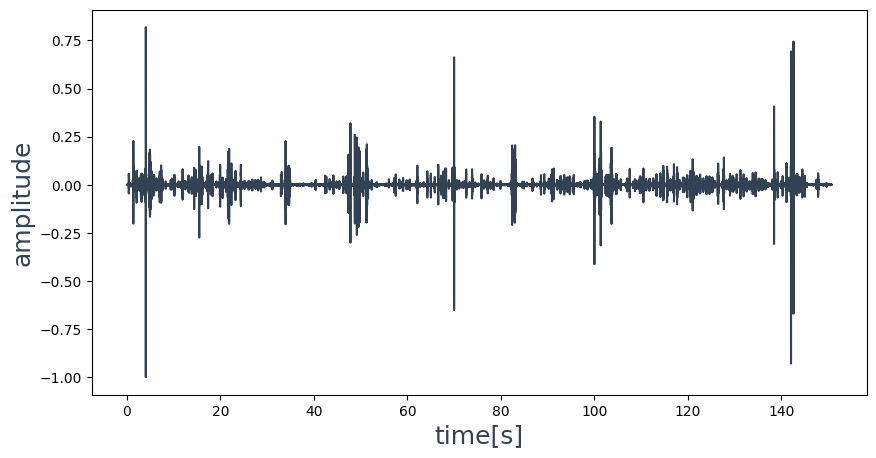
\includegraphics[width=1.0\hsize]{img/sound-example-rice.png}
            \subcaption{ご飯}
            \label{fig:sample-data-rice}
        \end{minipage}
        \\
        \\
        \begin{minipage}{0.6\hsize}
            \centering
            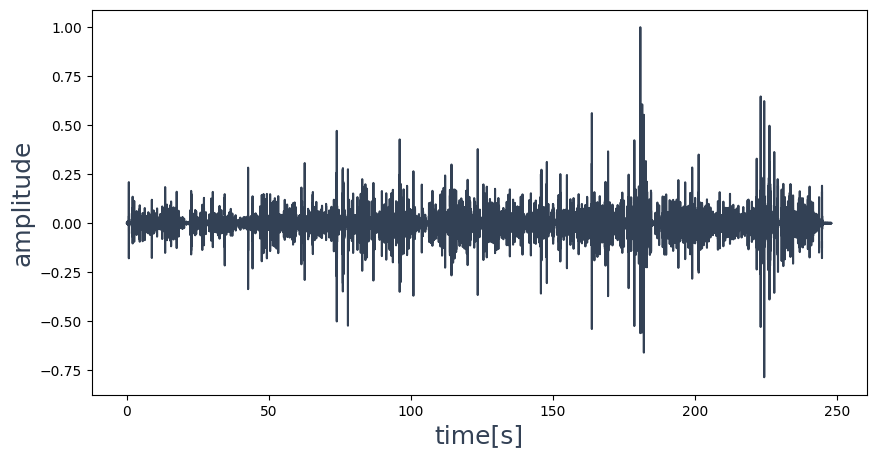
\includegraphics[width=1.0\hsize]{img/sound-example-salad.png}
            \subcaption{サラダ}
            \label{fig:sample-data-salad}
        \end{minipage}
        \\
        \\
        \begin{minipage}{0.6\hsize}
            \centering
            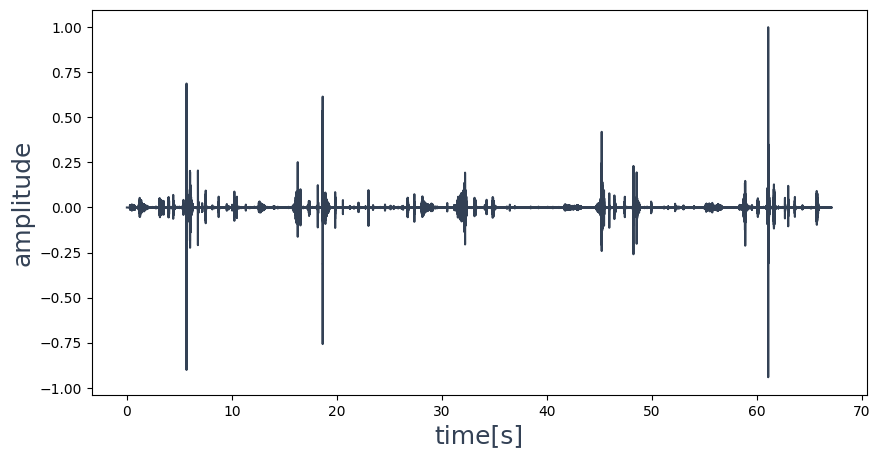
\includegraphics[width=1.0\hsize]{img/sound-example-soup.png}
            \subcaption{味噌汁}
            \label{fig:sample-data-soup}
        \end{minipage}
    \end{tabular}
    \caption{録音データの波形の一例}
    \label{fig:sample-data}
\end{figure}

\begin{figure}[t]
    \begin{center}
        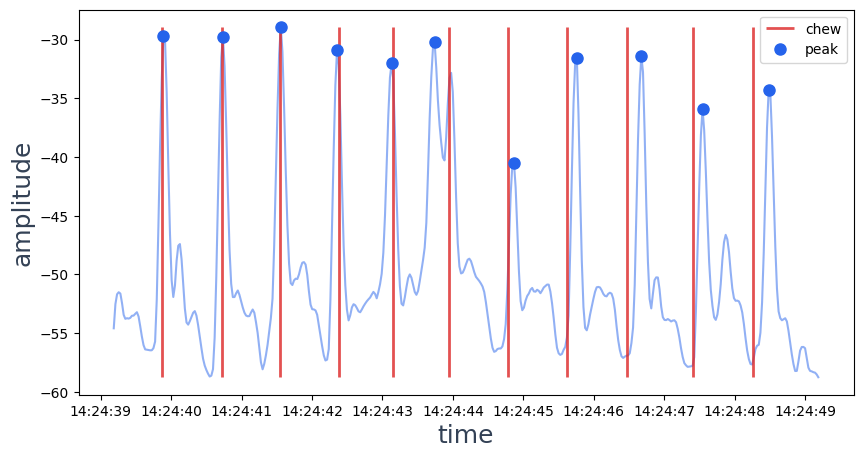
\includegraphics[clip,  width=0.95\hsize]{img/peak-sample.png}
        \caption{ピーク検出}
        \label{fig:peak-sample}
    \end{center}
\end{figure}

\begin{figure}[t]
    \begin{center}
        \includegraphics[clip,  width=0.95\hsize]{img/food.png}
        \caption{対象とする食品}
        \label{fig:foods}
    \end{center}
\end{figure}

%----------------------------------------------------------------------
\section{食事内容の推定}

本稿では, 食事中の録音データをメルスペクトログラムに変換し, 畳み込みニューラルネットワークによる学習を行うことで, 食事内容推定モデルを生成する. メルスペクトログラムを用いてCNNで音声分類を行うと従来の手法よりも精度が出ることが言われているため\cite{Dossou_2021_ICCV}, 本研究でもこの手法を採用する.
食事中に発生する音をウィンドウ幅$500ms$, オーバーラップ率$0.75$のスライディングウィンドウで部分時系列データに分割する. ただし, 最大信号強度が$-65dBFS$以下のデータと音の長さが$500ms$に満たないものは除外する. 特徴抽出のために, スライディングウィンドウでセグメントされた音データに対して, メルスペクトログラムを算出する. これらのデータを訓練データ$90\%$とテストデータ$10\%$に分割し, 訓練データを用いて畳み込みニューラルネットワークCNNを学習させる. CNNには4つの畳み込み層を使用し, 畳み込み層の後に一つの最大値プーリング層とドロップアウト層を使用する. 最後の層はソフトマックス層である. 最終的に, テストデータを用いて学習済みモデルの精度評価を行う.

%----------------------------------------------------------------------
\section{咀嚼の検出}

音声信号処理においてオンセット検出は一般的な手法であり, スペクトルエネルギ分布からピークを検出することで, 音楽イベントを自動で検出することができる. 本稿でも, 咀嚼イベントの検出にオンセット検出を採用する. 食事中の音をメルスペクトログラムに変換し, 各時間軸毎の全ての周波数帯の信号強度の平均を取り, ピークを検出することで, 咀嚼の検出を行う. 図\ref{fig:peak-sample}にピーク検出の例を示す. 評価については, 10秒間の音データに対して被験者がカウントした咀嚼回数とピーク検出回数との間の平均絶対値誤差$MAE$を算出する. $MAE$の算出式は以下に示す.

\begin{equation}
    \text{MAE} = \frac{1}{n} \sum_{i=1}^{n} | y_i - \hat{y}_i |
\end{equation}

\begin{table}[t]
    \centering
    \caption{被験者データ}
    \label{personaldata}
    \scalebox{0.85}{
        \begin{tabular}{c|c|c|c}
            \hline
            \textbf{被験者} & \textbf{年齢} & \textbf{性別} & \textbf{計測した食品}                                                                   \\ \hline\hline
            A            & 22          & 男           & \begin{tabular}{c}唐揚げ,クリームパン,グラタン\\ハンバーグ,ご飯,せんべい\\サラダ,味噌汁,焼きそば,ヨーグルト\end{tabular} \\ \hline
            B            & 23          & 男           & クッキー,ポテトチップス                                                                      \\ \hline
            C            & 22          & 男           & \begin{tabular}{c}クッキー,焼き魚,ハンバーグ\\スパゲティ,ヨーグルト\end{tabular}                        \\ \hline
            D            & 23          & 男           & クッキー,クリームパン,せんべい                                                                  \\ \hline
            E            & 23          & 男           & ご飯,サラダ,味噌汁,焼きそば                                                                   \\ \hline
            F            & 22          & 男           & クリームパン,ポテトチップス,サラダチキン                                                             \\ \hline
            G            & 27          & 男           & 唐揚げ,ご飯,サラダ,味噌汁                                                                    \\ \hline
            H            & 23          & 男           & ご飯,せんべい,味噌汁                                                                       \\ \hline
            I            & 22          & 男           & \begin{tabular}{c}唐揚げ,焼き魚,ハンバーグ\\ゼリー,味噌汁,焼きそば\end{tabular}                        \\ \hline
            J            & 26          & 男           & せんべい                                                                              \\ \hline
            K            & 22          & 男           & \begin{tabular}{c}焼き魚,ハンバーグ,スパゲティ\\サラダチキン,味噌汁,ヨーグルト\end{tabular}                  \\ \hline
            L            & 22          & 男           & グラタン,せんべい                                                                         \\ \hline
            M            & 21          & 男           & 唐揚げ,ご飯,サラダ,味噌汁                                                                    \\ \hline
            N            & 23          & 男           & ゼリー,ポテトチップス                                                                       \\ \hline
            O            & 22          & 男           & クッキー,せんべい                                                                         \\ \hline
        \end{tabular}
    }
\end{table}

\begin{figure*}[t]
    \begin{center}
        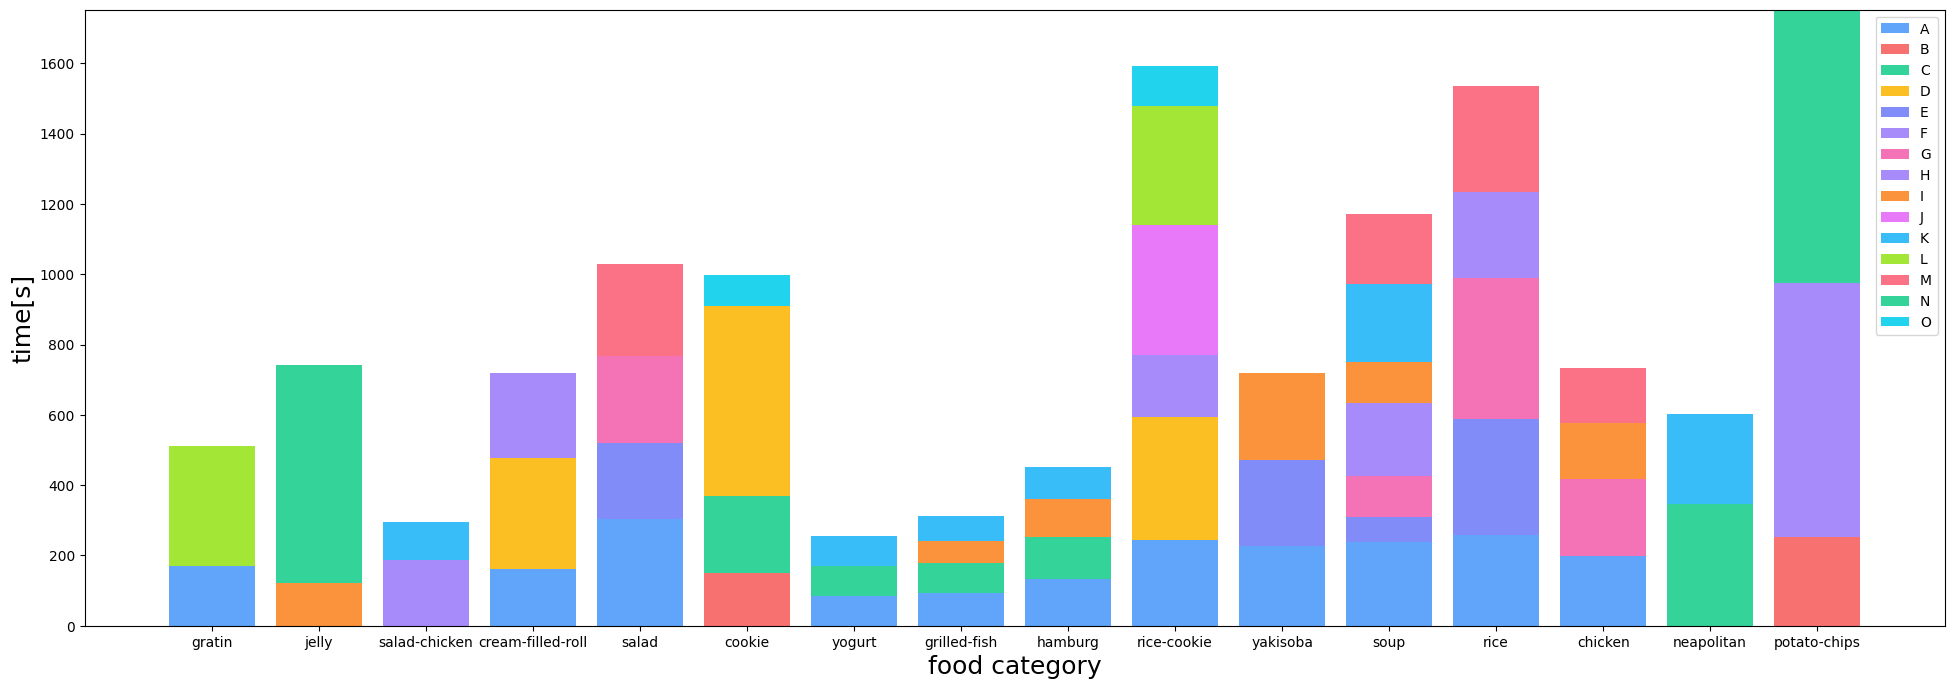
\includegraphics[clip,  width=0.9\hsize]{img/sound-data.png}
        \caption{食品毎の録音データ}
        \label{fig:sound-data}
    \end{center}
\end{figure*}

\begin{figure*}[t]
    \begin{minipage}[b]{0.16\hsize}
        \centering
        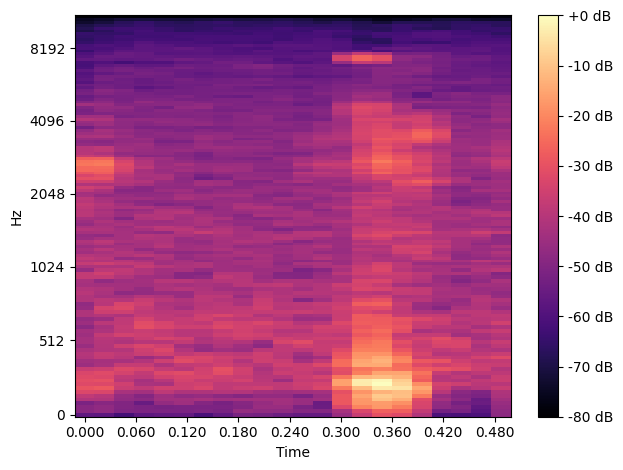
\includegraphics[width=\hsize]{img/melspec/chicken.png}
        \subcaption{唐揚げ}
    \end{minipage}
    \begin{minipage}[b]{0.16\hsize}
        \centering
        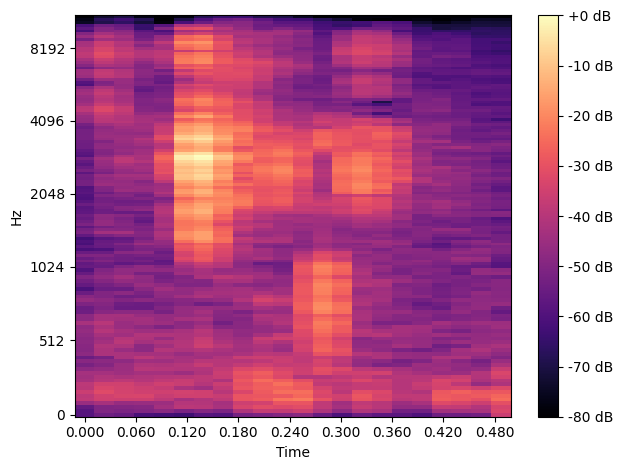
\includegraphics[width=\hsize]{img/melspec/rice.png}
        \subcaption{ご飯}
    \end{minipage}
    \begin{minipage}[b]{0.16\hsize}
        \centering
        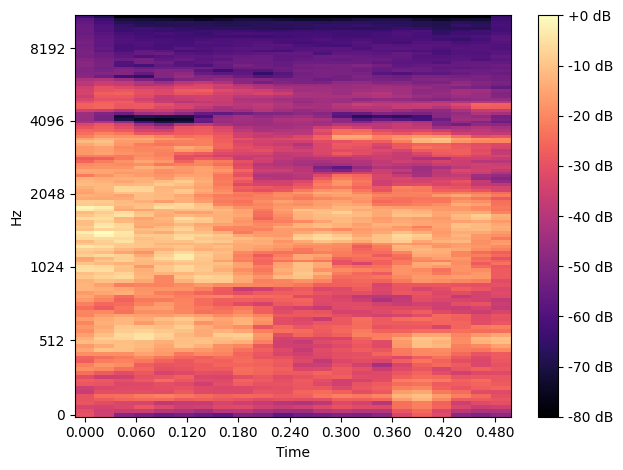
\includegraphics[width=\hsize]{img/melspec/soup.png}
        \subcaption{味噌汁}
    \end{minipage}
    \begin{minipage}[b]{0.16\hsize}
        \centering
        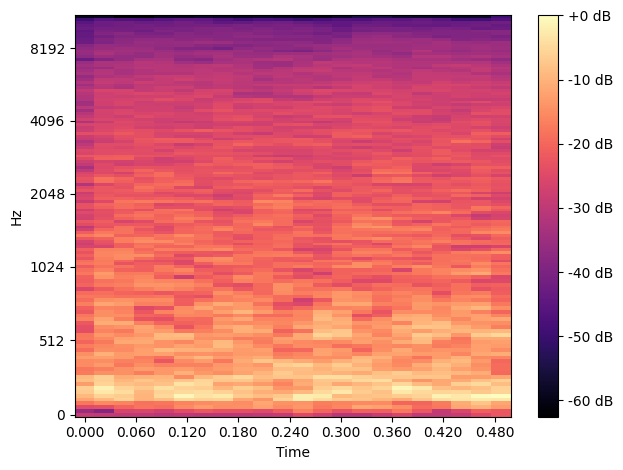
\includegraphics[width=\hsize]{img/melspec/salad.png}
        \subcaption{サラダ}
    \end{minipage}
    \begin{minipage}[b]{0.16\hsize}
        \centering
        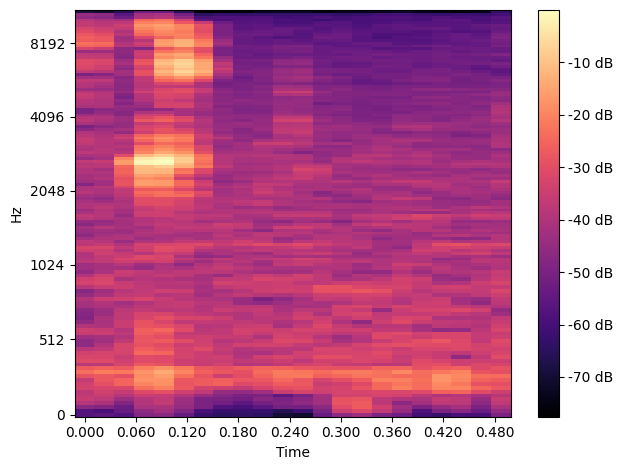
\includegraphics[width=\hsize]{img/melspec/rice-cookie.png}
        \subcaption{せんべい}
    \end{minipage}
    \begin{minipage}[b]{0.16\hsize}
        \centering
        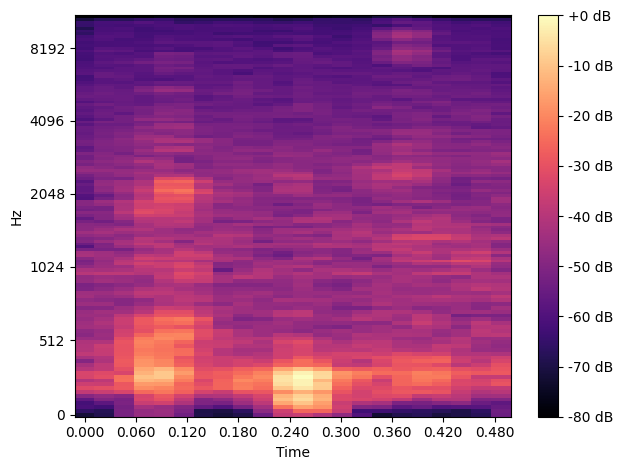
\includegraphics[width=\hsize]{img/melspec/gratin.png}
        \subcaption{グラタン}
    \end{minipage}
    \begin{minipage}[b]{0.16\hsize}
        \centering
        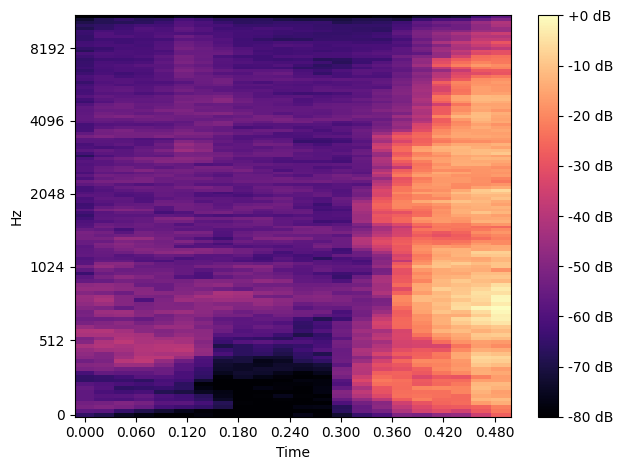
\includegraphics[width=\hsize]{img/melspec/cookie.png}
        \subcaption{クッキー}
    \end{minipage}
    \begin{minipage}[b]{0.16\hsize}
        \centering
        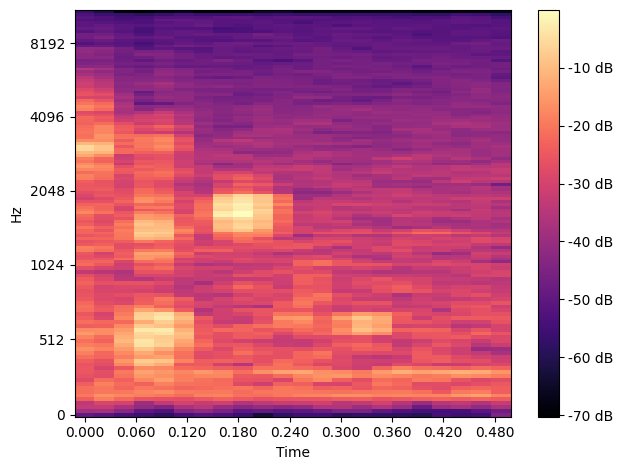
\includegraphics[width=\hsize]{img/melspec/potato-chips.png}
        \subcaption{ポテトチップス}
    \end{minipage}
    \begin{minipage}[b]{0.16\hsize}
        \centering
        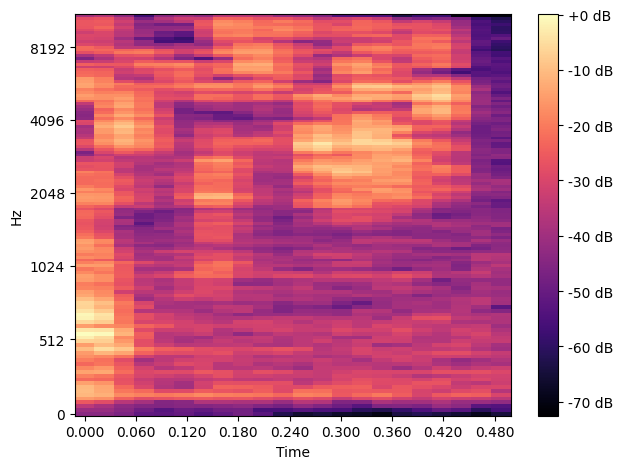
\includegraphics[width=\hsize]{img/melspec/neapolitan.png}
        \subcaption{スパゲティ}
    \end{minipage}
    \begin{minipage}[b]{0.16\hsize}
        \centering
        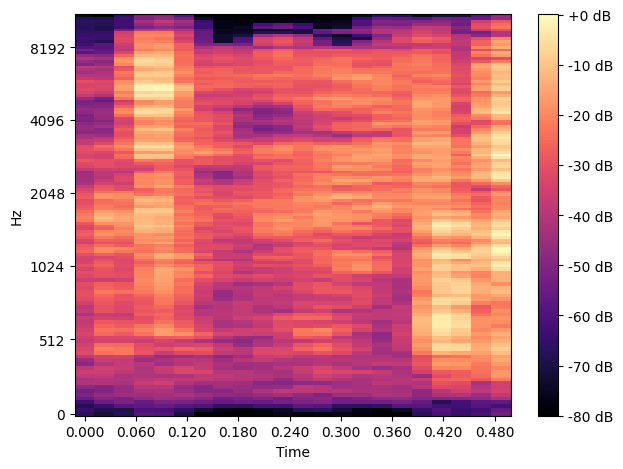
\includegraphics[width=\hsize]{img/melspec/yogurt.png}
        \subcaption{ヨーグルト}
    \end{minipage}
    \begin{minipage}[b]{0.16\hsize}
        \centering
        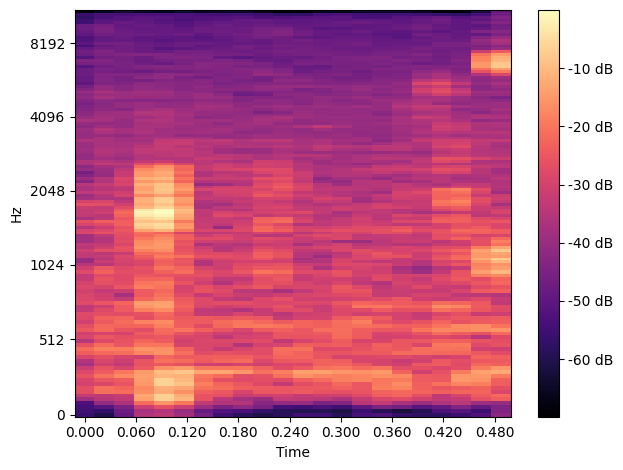
\includegraphics[width=\hsize]{img/melspec/hamburg.png}
        \subcaption{ハンバーグ}
    \end{minipage}
    \begin{minipage}[b]{0.16\hsize}
        \centering
        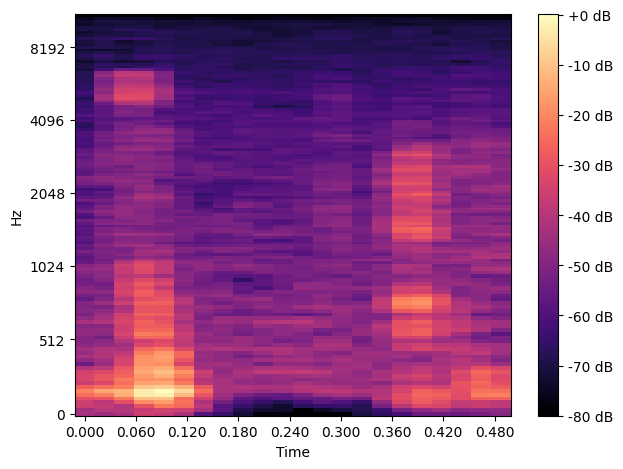
\includegraphics[width=\hsize]{img/melspec/salad-chicken.png}
        \subcaption{サラダチキン}
    \end{minipage}
    \begin{minipage}[b]{0.16\hsize}
        \centering
        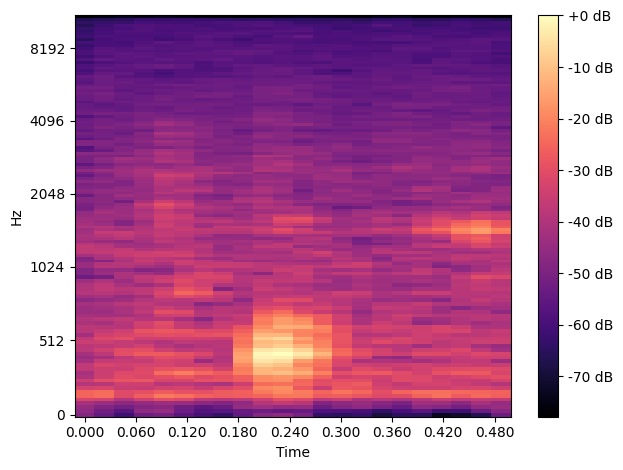
\includegraphics[width=\hsize]{img/melspec/cream-filled-roll.png}
        \subcaption{クリームパン}
    \end{minipage}
    \begin{minipage}[b]{0.16\hsize}
        \centering
        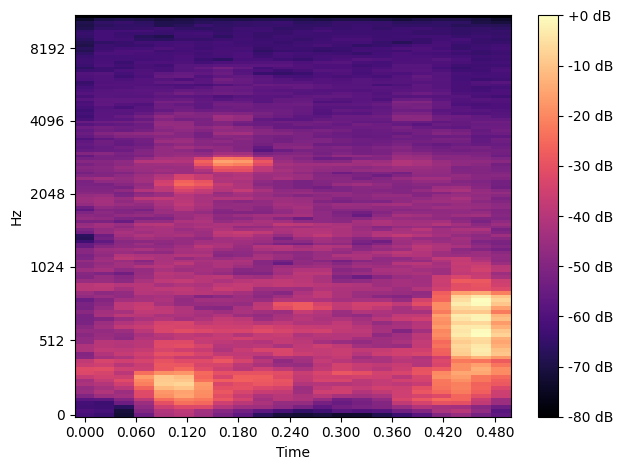
\includegraphics[width=\hsize]{img/melspec/yakisoba.png}
        \subcaption{焼きそば}
    \end{minipage}
    \begin{minipage}[b]{0.16\hsize}
        \centering
        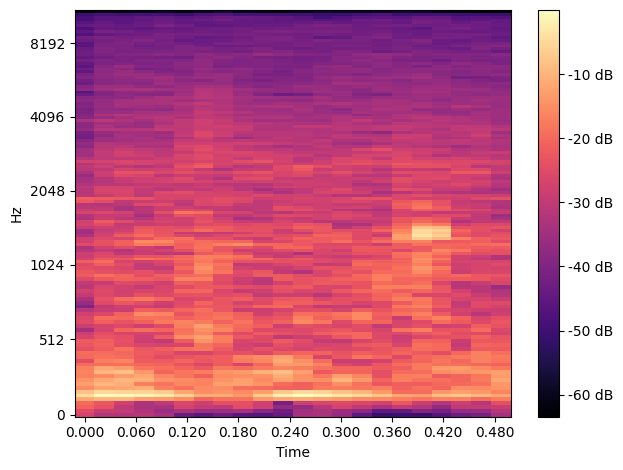
\includegraphics[width=\hsize]{img/melspec/jelly.png}
        \subcaption{ゼリー}
    \end{minipage}
    \begin{minipage}[b]{0.16\hsize}
        \centering
        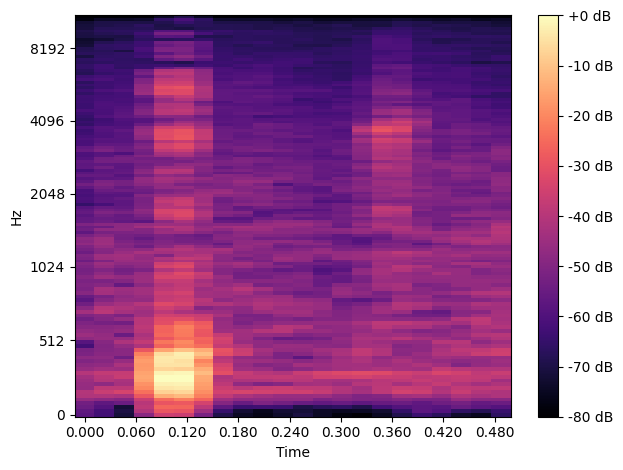
\includegraphics[width=\hsize]{img/melspec/grilled-fish.png}
        \subcaption{焼き魚}
    \end{minipage}
    \caption{録音データのメルスペクトログラムの一例}
    \label{fig:sample-melspec-data}
\end{figure*}

% 以下はRefTeX用
%%% Local Variables:
%%% mode: yatex
%%% TeX-master: "main"
%%% End:

%#! platex main.tex

%======================================================================
\chapter{評価実験}

本章では, 各食品毎の食事中の音を収集する実験を行う. その後, 収集した音データを分析し, 食事内容および咀嚼回数の推定を行なった.

\begin{figure}[t]
    \centering
    \begin{tabular}{c}
        \begin{minipage}{0.6\hsize}
            \centering
            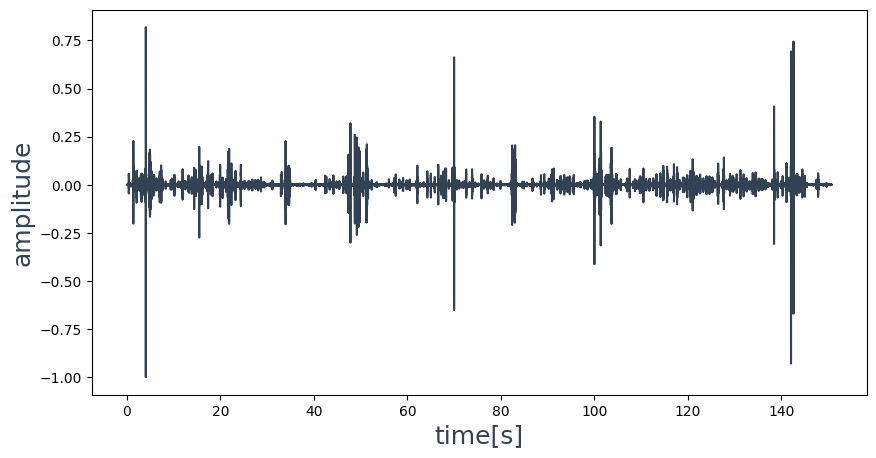
\includegraphics[width=1.0\hsize]{img/sound-example-rice.png}
            \subcaption{ご飯}
            \label{fig:sample-data-rice}
        \end{minipage}
        \\
        \\
        \begin{minipage}{0.6\hsize}
            \centering
            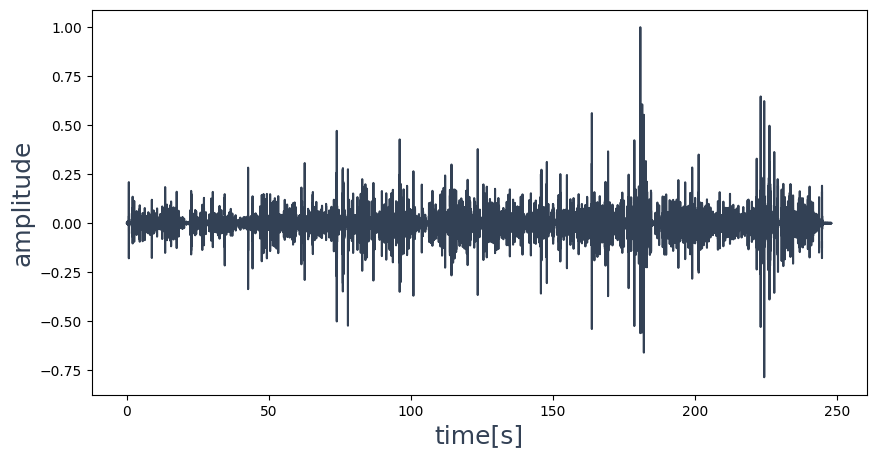
\includegraphics[width=1.0\hsize]{img/sound-example-salad.png}
            \subcaption{サラダ}
            \label{fig:sample-data-salad}
        \end{minipage}
        \\
        \\
        \begin{minipage}{0.6\hsize}
            \centering
            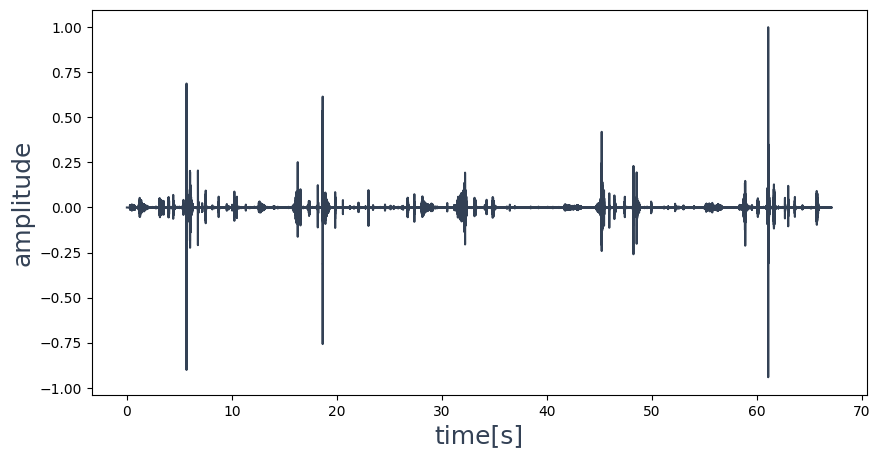
\includegraphics[width=1.0\hsize]{img/sound-example-soup.png}
            \subcaption{味噌汁}
            \label{fig:sample-data-soup}
        \end{minipage}
    \end{tabular}
    \caption{録音データの波形の一例}
    \label{fig:sample-data}
\end{figure}

\begin{figure}[t]
    \begin{center}
        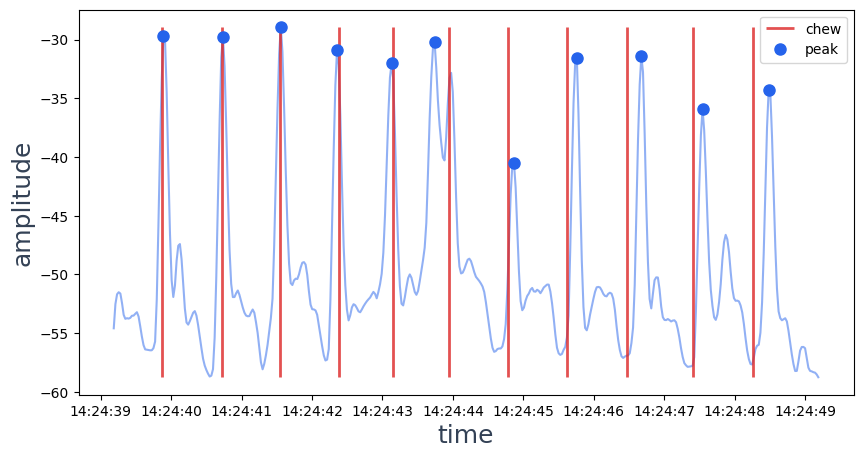
\includegraphics[clip,  width=0.95\hsize]{img/peak-sample.png}
        \caption{ピーク検出}
        \label{fig:peak-sample}
    \end{center}
\end{figure}

\begin{figure}[t]
    \begin{center}
        \includegraphics[clip,  width=0.95\hsize]{img/food.png}
        \caption{対象とする食品}
        \label{fig:foods}
    \end{center}
\end{figure}

\begin{table}[t]
    \centering
    \caption{被験者データ}
    \label{personaldata}
    \scalebox{0.85}{
        \begin{tabular}{c|c|c|c}
            \hline
            \textbf{被験者} & \textbf{年齢} & \textbf{性別} & \textbf{計測した食品}                                                                   \\ \hline\hline
            A            & 22          & 男           & \begin{tabular}{c}唐揚げ,クリームパン,グラタン\\ハンバーグ,ご飯,せんべい\\サラダ,味噌汁,焼きそば,ヨーグルト\end{tabular} \\ \hline
            B            & 23          & 男           & クッキー,ポテトチップス                                                                      \\ \hline
            C            & 22          & 男           & \begin{tabular}{c}クッキー,焼き魚,ハンバーグ\\スパゲティ,ヨーグルト\end{tabular}                        \\ \hline
            D            & 23          & 男           & クッキー,クリームパン,せんべい                                                                  \\ \hline
            E            & 23          & 男           & ご飯,サラダ,味噌汁,焼きそば                                                                   \\ \hline
            F            & 22          & 男           & クリームパン,ポテトチップス,サラダチキン                                                             \\ \hline
            G            & 27          & 男           & 唐揚げ,ご飯,サラダ,味噌汁                                                                    \\ \hline
            H            & 23          & 男           & ご飯,せんべい,味噌汁                                                                       \\ \hline
            I            & 22          & 男           & \begin{tabular}{c}唐揚げ,焼き魚,ハンバーグ\\ゼリー,味噌汁,焼きそば\end{tabular}                        \\ \hline
            J            & 26          & 男           & せんべい                                                                              \\ \hline
            K            & 22          & 男           & \begin{tabular}{c}焼き魚,ハンバーグ,スパゲティ\\サラダチキン,味噌汁,ヨーグルト\end{tabular}                  \\ \hline
            L            & 22          & 男           & グラタン,せんべい                                                                         \\ \hline
            M            & 21          & 男           & 唐揚げ,ご飯,サラダ,味噌汁                                                                    \\ \hline
            N            & 23          & 男           & ゼリー,ポテトチップス                                                                       \\ \hline
            O            & 22          & 男           & クッキー,せんべい                                                                         \\ \hline
        \end{tabular}
    }
\end{table}

\begin{figure*}[t]
    \begin{center}
        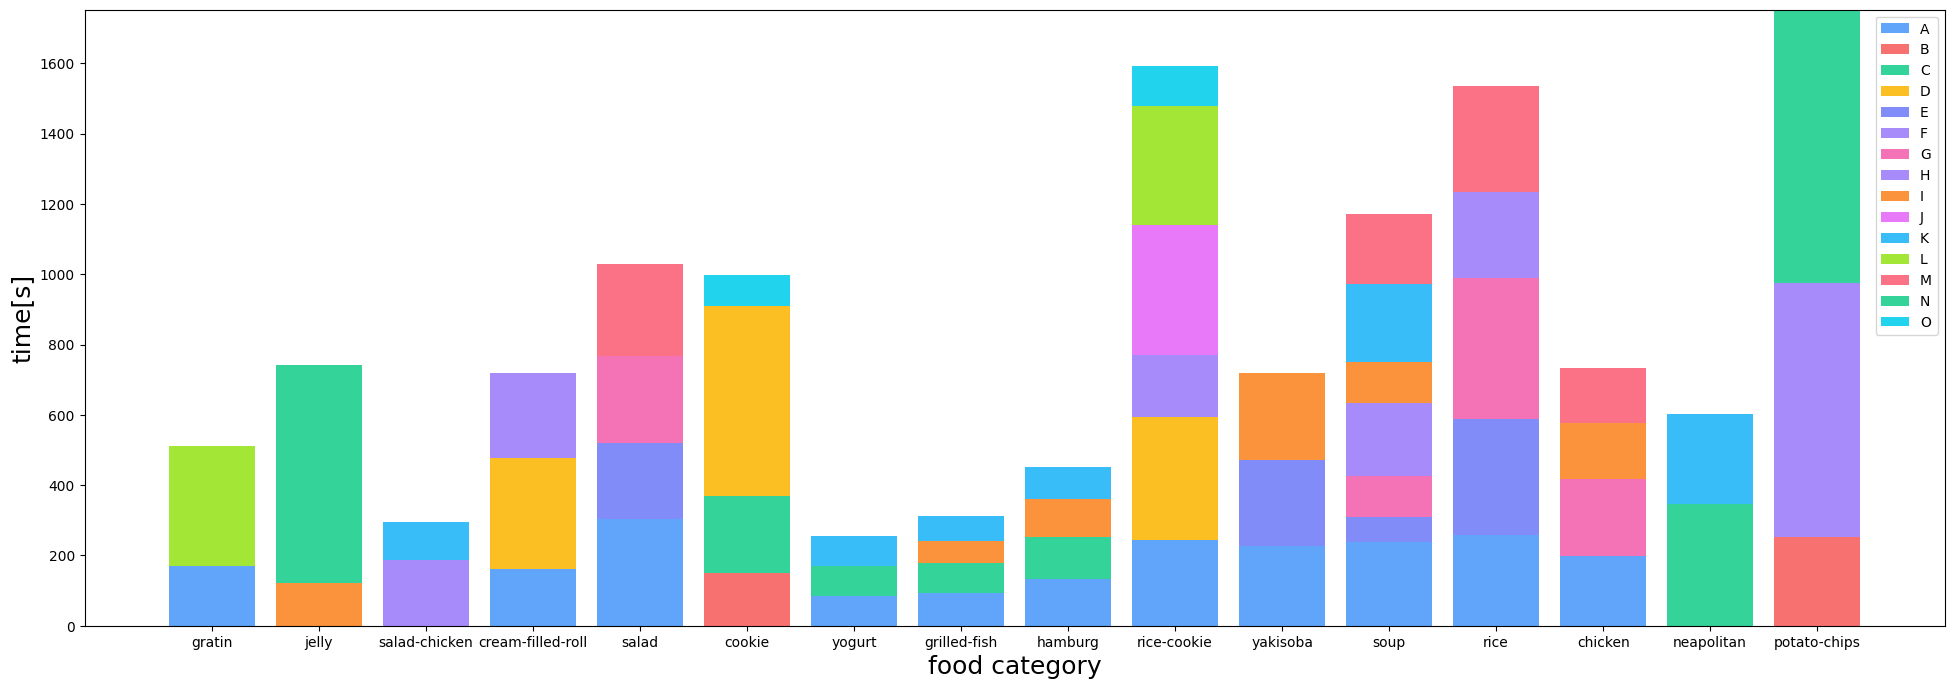
\includegraphics[clip,  width=0.9\hsize]{img/sound-data.png}
        \caption{食品毎の録音データ}
        \label{fig:sound-data}
    \end{center}
\end{figure*}

% \begin{figure*}[t]
%     \begin{minipage}[b]{0.16\hsize}
%         \centering
%         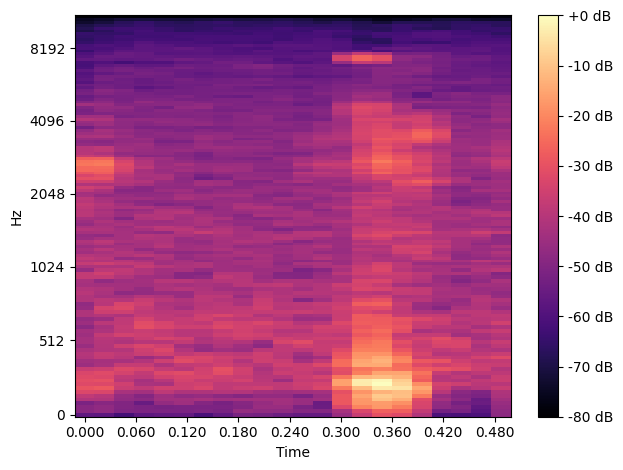
\includegraphics[width=\hsize]{img/melspec/chicken.png}
%         \subcaption{唐揚げ}
%     \end{minipage}
%     \begin{minipage}[b]{0.16\hsize}
%         \centering
%         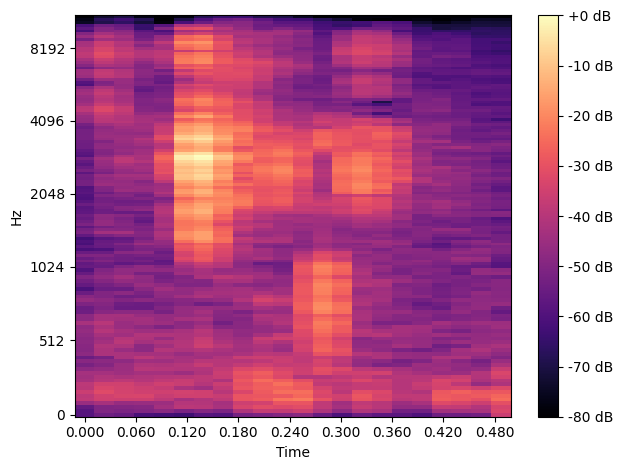
\includegraphics[width=\hsize]{img/melspec/rice.png}
%         \subcaption{ご飯}
%     \end{minipage}
%     \begin{minipage}[b]{0.16\hsize}
%         \centering
%         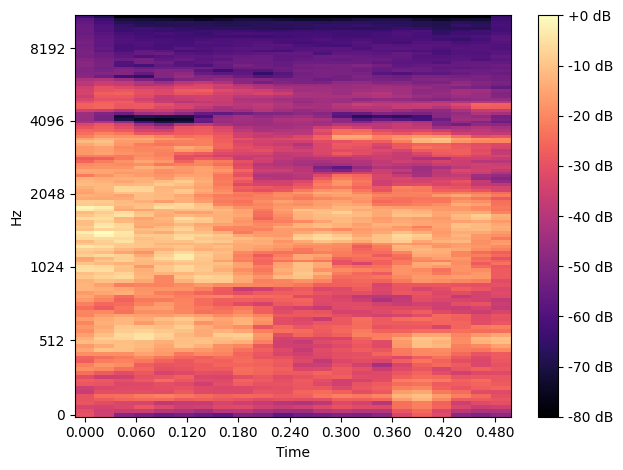
\includegraphics[width=\hsize]{img/melspec/soup.png}
%         \subcaption{味噌汁}
%     \end{minipage}
%     \begin{minipage}[b]{0.16\hsize}
%         \centering
%         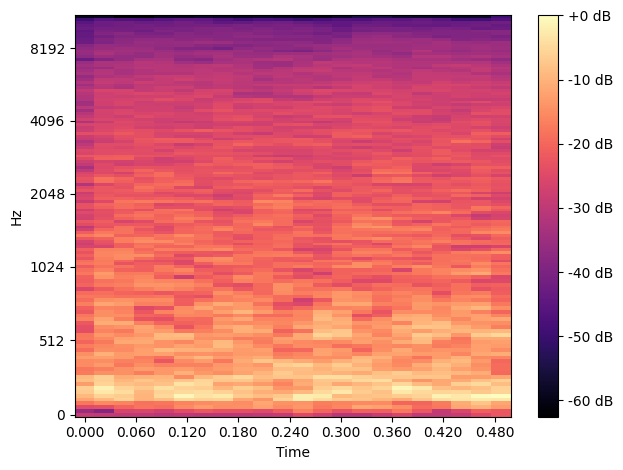
\includegraphics[width=\hsize]{img/melspec/salad.png}
%         \subcaption{サラダ}
%     \end{minipage}
%     \begin{minipage}[b]{0.16\hsize}
%         \centering
%         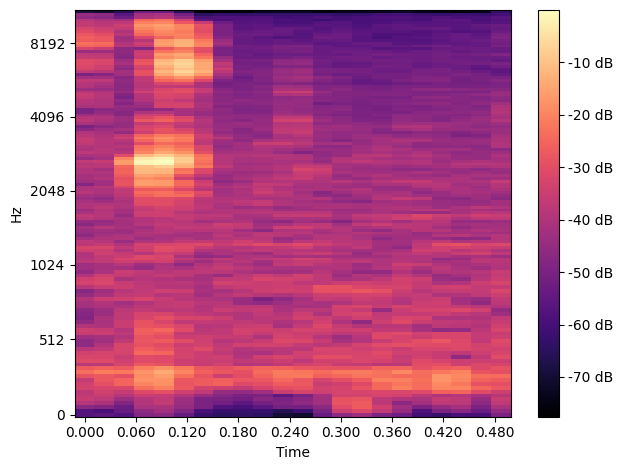
\includegraphics[width=\hsize]{img/melspec/rice-cookie.png}
%         \subcaption{せんべい}
%     \end{minipage}
%     \begin{minipage}[b]{0.16\hsize}
%         \centering
%         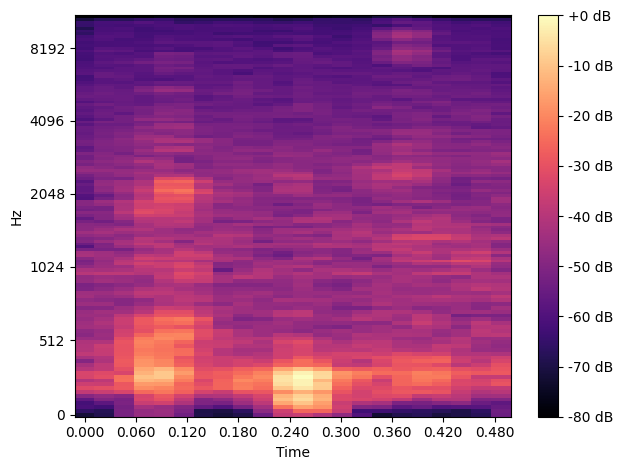
\includegraphics[width=\hsize]{img/melspec/gratin.png}
%         \subcaption{グラタン}
%     \end{minipage}
%     \begin{minipage}[b]{0.16\hsize}
%         \centering
%         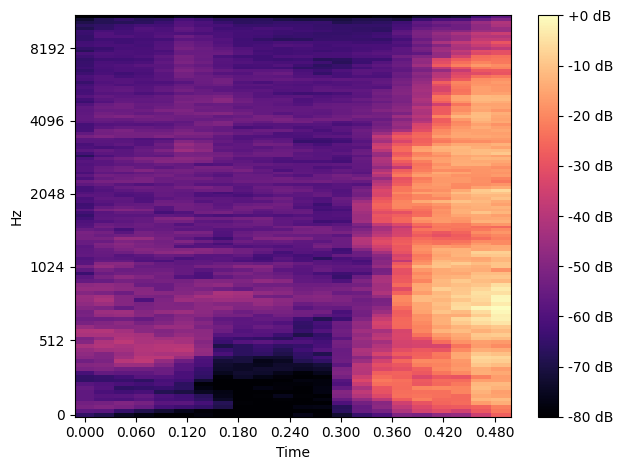
\includegraphics[width=\hsize]{img/melspec/cookie.png}
%         \subcaption{クッキー}
%     \end{minipage}
%     \begin{minipage}[b]{0.16\hsize}
%         \centering
%         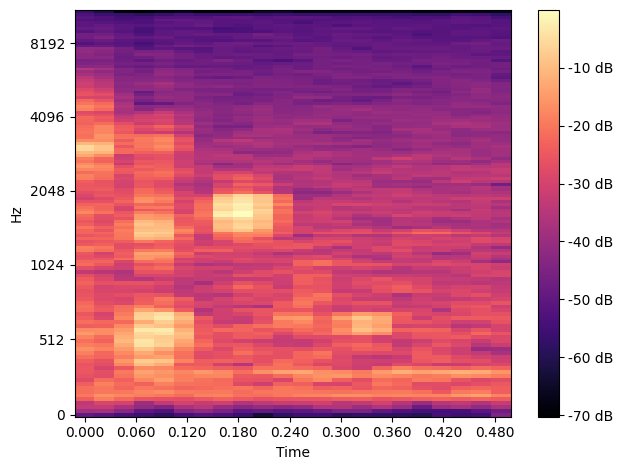
\includegraphics[width=\hsize]{img/melspec/potato-chips.png}
%         \subcaption{ポテトチップス}
%     \end{minipage}
%     \begin{minipage}[b]{0.16\hsize}
%         \centering
%         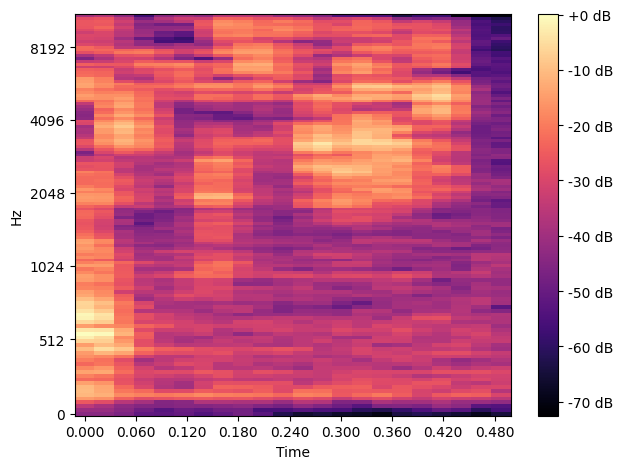
\includegraphics[width=\hsize]{img/melspec/neapolitan.png}
%         \subcaption{スパゲティ}
%     \end{minipage}
%     \begin{minipage}[b]{0.16\hsize}
%         \centering
%         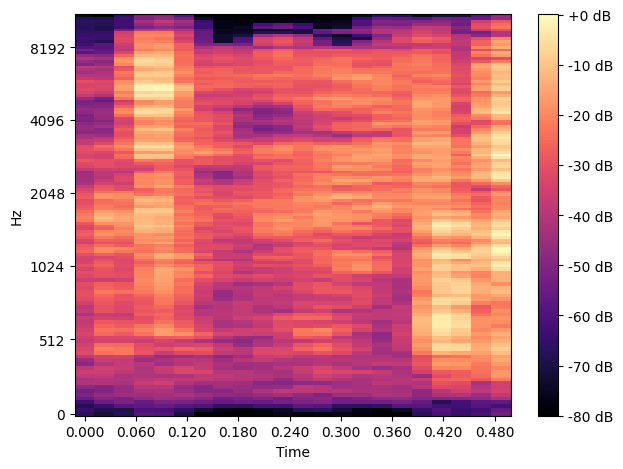
\includegraphics[width=\hsize]{img/melspec/yogurt.png}
%         \subcaption{ヨーグルト}
%     \end{minipage}
%     \begin{minipage}[b]{0.16\hsize}
%         \centering
%         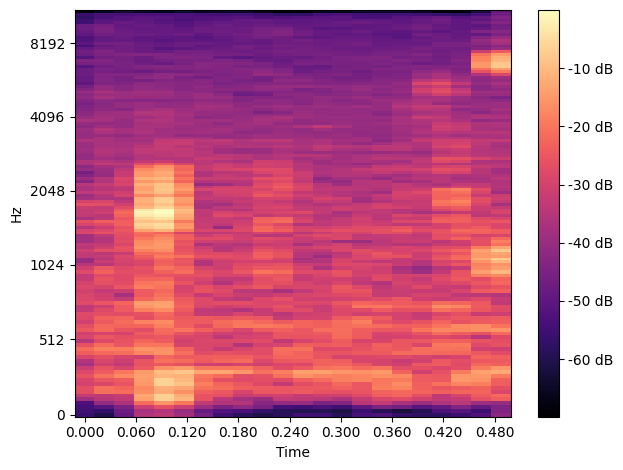
\includegraphics[width=\hsize]{img/melspec/hamburg.png}
%         \subcaption{ハンバーグ}
%     \end{minipage}
%     \begin{minipage}[b]{0.16\hsize}
%         \centering
%         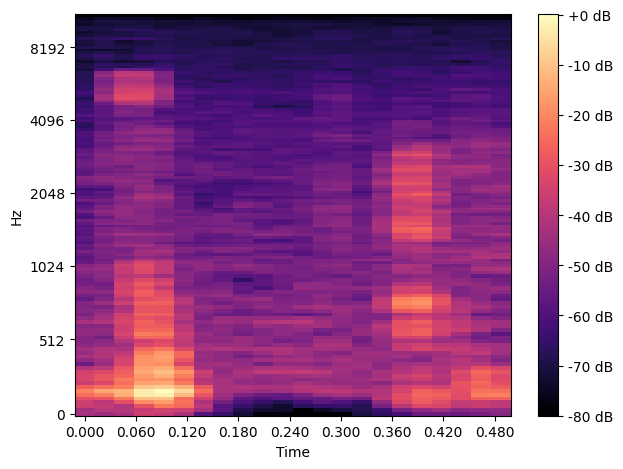
\includegraphics[width=\hsize]{img/melspec/salad-chicken.png}
%         \subcaption{サラダチキン}
%     \end{minipage}
%     \begin{minipage}[b]{0.16\hsize}
%         \centering
%         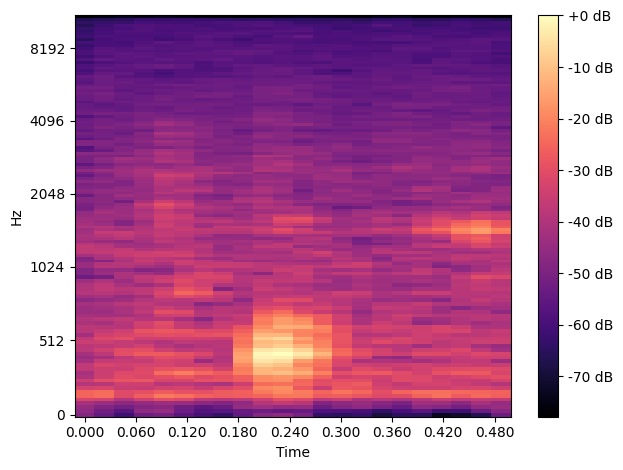
\includegraphics[width=\hsize]{img/melspec/cream-filled-roll.png}
%         \subcaption{クリームパン}
%     \end{minipage}
%     \begin{minipage}[b]{0.16\hsize}
%         \centering
%         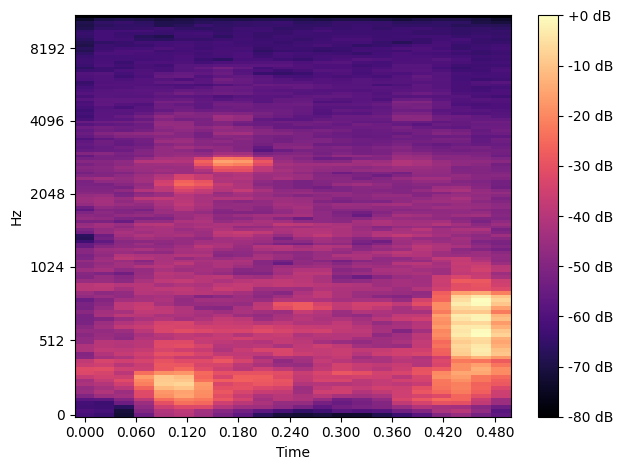
\includegraphics[width=\hsize]{img/melspec/yakisoba.png}
%         \subcaption{焼きそば}
%     \end{minipage}
%     \begin{minipage}[b]{0.16\hsize}
%         \centering
%         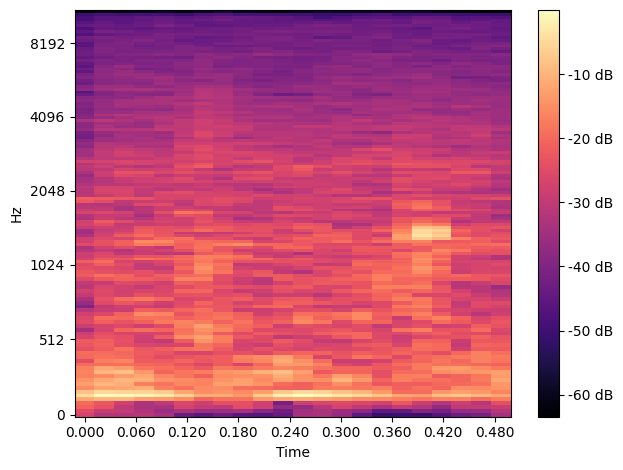
\includegraphics[width=\hsize]{img/melspec/jelly.png}
%         \subcaption{ゼリー}
%     \end{minipage}
%     \begin{minipage}[b]{0.16\hsize}
%         \centering
%         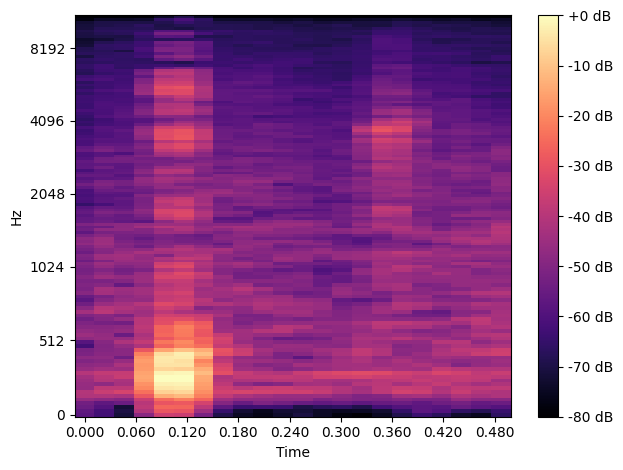
\includegraphics[width=\hsize]{img/melspec/grilled-fish.png}
%         \subcaption{焼き魚}
%     \end{minipage}
%     \caption{録音データのメルスペクトログラムの一例}
%     \label{fig:sample-melspec-data}
% \end{figure*}

%----------------------------------------------------------------------
\section{対象とする食事}

図\ref{fig:foods}に示すように, 本研究において対象とする食品は以下の16種類である. 基本的には, 一般的な日本人がよく食べる食品を中心にピックアップしており, 柔らかいものから固いものまで多岐に渡る.

\begin{itemize}
    \item 唐揚げ
    \item ご飯
    \item 味噌汁
    \item サラダ
    \item せんべい
    \item グラタン
    \item クッキー
    \item ポテトチップス
    \item スパゲティ
    \item ヨーグルト
    \item ハンバーグ
    \item サラダチキン
    \item クリームパン
    \item 焼きそば
    \item ゼリー
    \item 焼き魚
\end{itemize}

また録音データの一例として, 図\ref{fig:sample-data}にAirPodsによって計測された録音データの波形を示す.

%----------------------------------------------------------------------
\section{実験準備}

本研究では, Apple社製のAirPodsシリーズ\footnote{AirPods - Apple~\url{https://www.apple.com/jp/airpods/}}を用いて録音を行う. AirPodsシリーズには, AirPodsの第1世代から第3世代, AirPods Proの第1世代から第2世代までのラインナップがあり, 全てのモデルにおいて, 内臓マイクが搭載されている. 評価実験は, 環境音の少ない静かな環境で, 21〜27歳の15名の被験者(\tablename\ref{personaldata})によって行われた. 被験者は, AirPodsを耳に装着し, アプリケーションで測定を開始した上で, 食事を行った. 計測は一品ずつ行い, 食品を変える際は一回計測を終了してから再度計測をしなおすことで, 1つの音データには1種類の食事のみを含むようにした. その結果, 合計13422秒の食事中の録音データを記録することができた. 図\ref{fig:sound-data}は, 食品毎の録音データの録音時間の累計を示す.

\begin{table}[t]
    \centering
    \caption{食品毎の食事内容推定モデルの精度}
    \label{result}
    \scalebox{0.9}{
        \begin{tabular}{c|c|c|c|c}
            \hline
            \textbf{食品} & \textbf{precision} & \textbf{recall} & \textbf{f1-score} & \textbf{support} \\ \hline\hline
            ポテトチップス     & 0.88               & 0.91            & 0.90              & 1409.0           \\ \hline
            クリームパン      & 0.87               & 0.86            & 0.86              & 488.0            \\ \hline
            せんべい        & 0.87               & 0.83            & 0.85              & 1229.0           \\ \hline
            ゼリー         & 0.84               & 0.82            & 0.83              & 512.0            \\ \hline
            スパゲティ       & 0.90               & 0.72            & 0.80              & 454.0            \\ \hline
            サラダ         & 0.76               & 0.81            & 0.79              & 834.0            \\ \hline
            焼きそば        & 0.79               & 0.78            & 0.78              & 556.0            \\ \hline
            クッキー        & 0.80               & 0.75            & 0.77              & 787.0            \\ \hline
            グラタン        & 0.79               & 0.76            & 0.77              & 381.0            \\ \hline
            サラダチキン      & 0.80               & 0.68            & 0.74              & 232.0            \\ \hline
            味噌汁         & 0.75               & 0.69            & 0.72              & 900.0            \\ \hline
            ご飯          & 0.62               & 0.80            & 0.70              & 1170.0           \\ \hline
            ヨーグルト       & 0.68               & 0.64            & 0.66              & 165.0            \\ \hline
            唐揚げ         & 0.67               & 0.57            & 0.62              & 581.0            \\ \hline
            ハンバーグ       & 0.59               & 0.62            & 0.60              & 317.0            \\ \hline
            焼き魚         & 0.54               & 0.54            & 0.54              & 218.0            \\ \hline
        \end{tabular}
    }
\end{table}

\begin{figure}[t]
    \begin{center}
        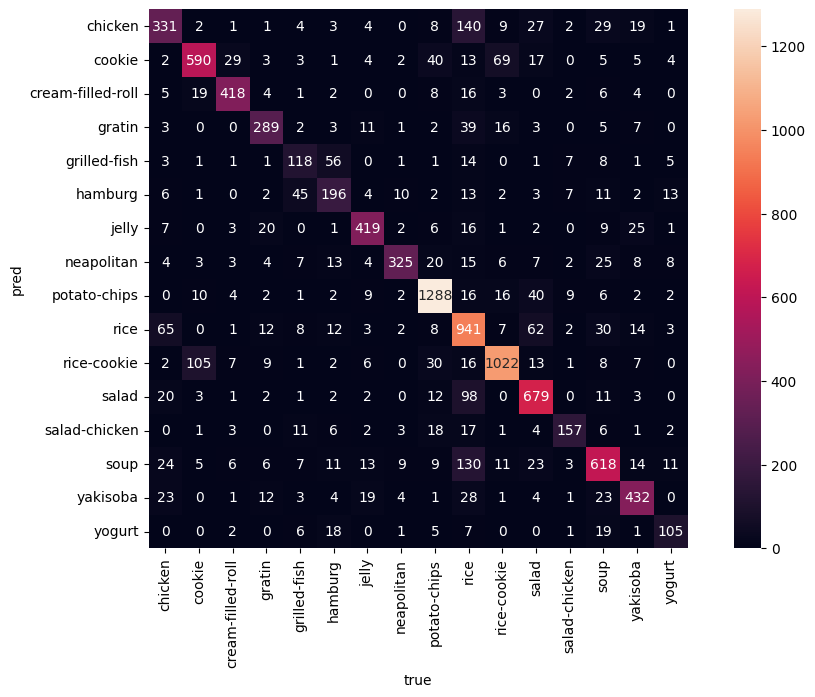
\includegraphics[clip,  width=0.95\hsize]{img/confusion_matrix.png}
        \caption{食事内容推定モデルの混合行列}
        \label{fig:confusion-matrix}
    \end{center}
\end{figure}

%----------------------------------------------------------------------
\section{食事内容の推定}

AirPodsから44100Hzのサンプリング周波数で取得された録音データをスライディングウィンドウで部分時系列データに分割する. その結果, 107421件の音データを得ることができた. ただし, 最大信号強度が$-65dBFS$以下のデータと音の長さが$500ms$に満たないものは除外したため, 最終的に使用したデータは102960件である.

これらのデータを用いて, 食事内容推定モデルを学習させたところ, テストデータに対して, 精度$77.5\%$という結果となった. \tablename\ref{result}に食品毎の精度を示す. F1スコアを比較すると, ポテトチップスが一番精度が高く, 焼き魚が一番精度が低いことがわかる. また, 図\ref{fig:confusion-matrix}に混合行列を示す. 混合行列から, クッキーがせんべいと誤判定したり, 逆にせんべいがクッキーと誤判定しやすいことがわかる. これは, どちらも食べ物の形状が同じで, 食感も硬く, 食品としての特徴が似ているからであると考えられる. また, ご飯以外の全ての食品が誤ってご飯と判定する傾向があることがわかる. これは, 全ての咀嚼に共通するクチャクチャ音とご飯を咀嚼するときの音がどちらもやや高音で, 特徴が似ているからではないかと考える.

\begin{table}[t]
    \centering
    \caption{食品毎の咀嚼回数検出の精度}
    \label{result-chews}
    \scalebox{0.85} {
        \begin{tabular}{c|c|c|c|c}
            \hline
            \textbf{食品} & \textbf{MAE} & \begin{tabular}{c}\textbf{amplitude}\\\textbf{[dBFS]}\end{tabular} & \begin{tabular}{c}\textbf{chew}\\\textbf{count}\end{tabular} & \begin{tabular}{c}\textbf{peak}\\\textbf{count}\end{tabular} \\ \hline\hline
            せんべい        & 2.68         & -69.5                                                                                              & 9.89                                                         & 12.11                                                        \\ \hline
            クッキー        & 2.81         & -73.4                                                                                              & 10.83                                                        & 12.92                                                        \\ \hline
            グラタン        & 3.67         & -78.3                                                                                              & 5.22                                                         & 8.30                                                         \\ \hline
            スパゲティ       & 3.89         & -69.2                                                                                              & 8.66                                                         & 12.02                                                        \\ \hline
            サラダチキン      & 3.89         & -76.5                                                                                              & 13.92                                                        & 10.75                                                        \\ \hline
            ヨーグルト       & 4.29         & -75.1                                                                                              & 3.38                                                         & 9.50                                                         \\ \hline
            ポテトチップス     & 4.39         & -71.6                                                                                              & 11.58                                                        & 13.82                                                        \\ \hline
            サラダ         & 4.72         & -68.9                                                                                              & 11.61                                                        & 16.89                                                        \\ \hline
            ハンバーグ       & 5.80         & -78.4                                                                                              & 12.26                                                        & 8.52                                                         \\ \hline
            焼きそば        & 5.87         & -73.7                                                                                              & 10.56                                                        & 10.16                                                        \\ \hline
            唐揚げ         & 6.33         & -74.5                                                                                              & 12.66                                                        & 9.16                                                         \\ \hline
            ご飯          & 6.45         & -75.7                                                                                              & 11.26                                                        & 7.42                                                         \\ \hline
            クリームパン      & 6.72         & -80.0                                                                                              & 10.24                                                        & 3.55                                                         \\ \hline
            ゼリー         & 6.90         & -79.9                                                                                              & 8.93                                                         & 4.50                                                         \\ \hline
            焼き魚         & 7.64         & -79.7                                                                                              & 12.90                                                        & 7.70                                                         \\ \hline
        \end{tabular}
    }
\end{table}

%----------------------------------------------------------------------
\section{咀嚼回数の推定結果}

ピーク検出数つまり推定咀嚼回数と被験者がカウントした咀嚼回数の間では$MAE = 4.9$となった. つまり, ピーク検出による推定の咀嚼回数と実際の咀嚼回数との間には, 平均4.9回の誤差が発生する結果となった. しかし, \tablename\ref{result-chews}に示すように, 食品間で$MAE$にばらつきがあることがわかる. \tablename\ref{result-chews}には, $MAE$の他に平均振幅(amplitude[dBFS])・被験者のカウントした咀嚼回数の平均値(chew count)・平均ピーク検出数(peak count)を示す. せんべいやクッキーの精度が高くなったのは, 今回の対象の食品の中でも特に食感の硬い食べ物であり, 咀嚼音がはっきりと発生したからであると考えられる. 平均振幅に着目すると, 基本的に振幅の大きいものは誤差が少ない傾向があることがわかる. しかし, サラダやポテトチップスは平均振幅が大きい部類であるが, 誤差がやや大きいことがわかる. これは, 被験者がカウントした咀嚼回数に比べてピーク検出回数が多いことから, 実際の咀嚼回数が多く, 被験者自身が全ての咀嚼をカウントすることができなかったのではないかと考えられる.

%#! platex main.tex

%======================================================================
\chapter{食事行動改善のためのフィードバックシステム}
\label{cha:intervention}

先ほどの章まででは, 食事中の音から食品認識や咀嚼検出を行う手法を提案してきた. 本章では, これらのセンシング手法を用いて食事行動を分析し, 健康的な食事を促進するためのフィードバックシステムについて提案する. 健康的な食事を促進するシステムとして代表的なものは, カロミルやあすけんといった食事管理アプリケーションである. 食事の写真から食品認識を行い, カロリやタンパク質などの栄養素を自動で計算することができ, 日々の食事のバランスを見直すきっかけになる. さらにカロミルでは, 食事・運動・アプリの起動状況などから3ヶ月後の体重を予測する機能も搭載されている. これらのアプリケーションは, スマートフォンのカメラで食事の写真を撮影するだけで利用することができるといった手軽さから広く普及している. しかし, 冒頭でも述べた通り, 食事の内容だけでなく, 食べる順番や速度などの食事行動に関しても, 健康的な食生活を送る上で非常に大切ではある. しかしながら, 既存の食事管理アプリケーションでは, あくまで食事の内容に対する評価しか行うことができない. シャープが開発したbitescanでは, 独自の耳掛け式のウェアラブルデバイスを用いて, 食事中にリアルタイムで咀嚼回数と一口あたりの回数をアプリケーションの画面を通じて確認することができる. さらに, 咀嚼回数やテンポなどが数値化されることで, 自身の食事行動を振り返ることができる. しかし, 独自のウェアラブルデバイスが必要となるため, 普及性に課題があり, そもそも咀嚼回数のみを計測しているため, 食べる順番に対する評価を行うことができない. また, 食べる順番や速度などをアドバイスするために, ウェアラブルデバイスで食事行動を撮影した一人称映像から食事内容をリアルタイムで検出する研究も存在する. しかし, この手法も食事中にカメラで撮影し続ける必要があるため, 一般的な食事シーンで計測を行うのは受け入れ難い. 我々の研究グループでは, 健康的な食生活を促進する行動変容システムとしてeat2picを提案している.\cite{10.1145/3580784} 本研究では, イヤラブルデバイスから食事行動をセンシングし, フィードバックを行うシステムの一例として, eat2picのナッジメカニズムをベースにした咀嚼音から絵を描く「Chew-Draw」インタラクションを提案する.

\begin{figure}[t]
    \begin{center}
        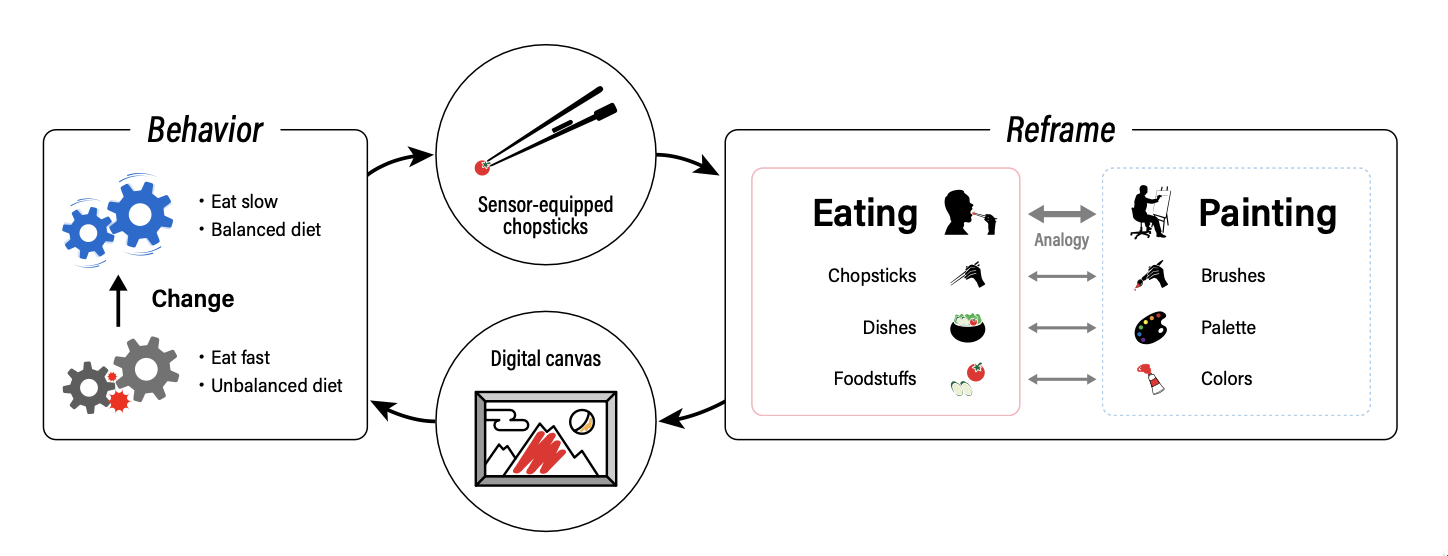
\includegraphics[clip, width=1.0\hsize]{img/eat2pic-concept.png}
        \caption{eat2picのコンセプト}
        \label{fig:eat2pic-concept}
    \end{center}
\end{figure}

\begin{figure}[t]
    \begin{center}
        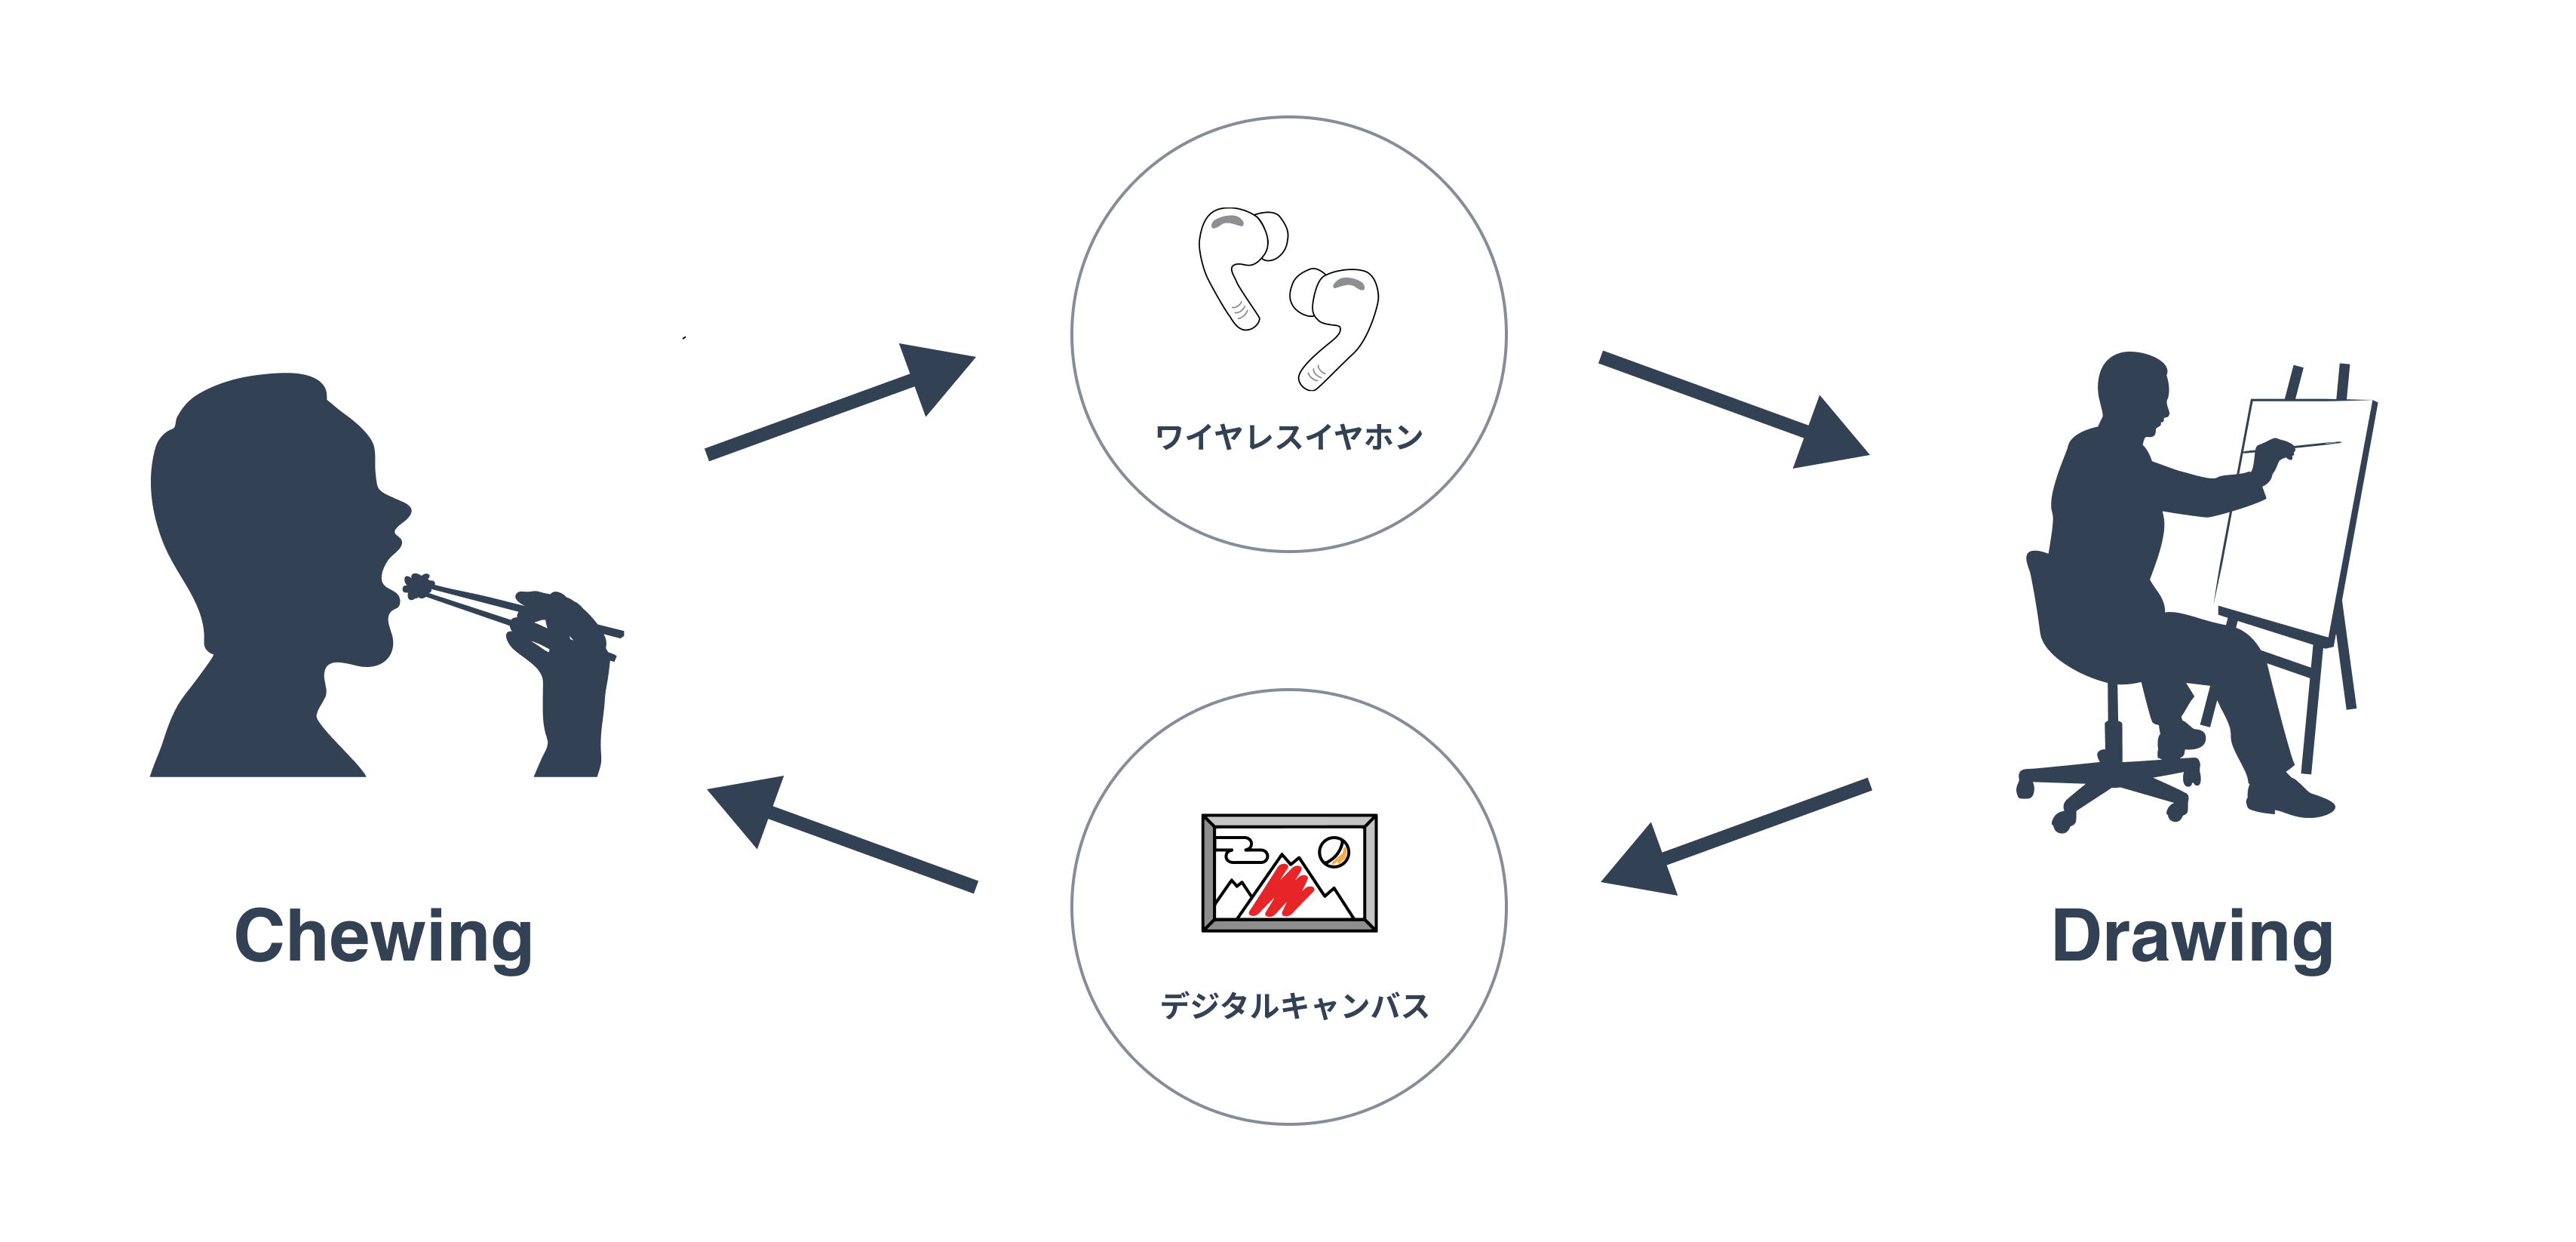
\includegraphics[clip, width=1.0\hsize]{img/chew-draw.png}
        \caption{Chew-Drawインタラクション}
        \label{fig:chew-draw}
    \end{center}
\end{figure}

\section{Chew-Drawインタラクション}

物理世界における「食べる」行動をモニタリングし, それをデジタルな「描く」世界に反映させるナッジングシステム, つまり「食べる」から「描く」をデザインしたeat2picの設計を踏襲する. 図\ref{fig:eat2pic-concept}は, eat2picのコンセプトデザインの概要である. eat2picでは, ほとんどの人が健康的な食習慣を身につけていないのは, 個人的な動機付けの不足, および個人的な成果空間の中での促しが不十分であると仮説を立て, 食べるタスクを他の遊びのタスクに置き換えることでユーザのモチベーションに影響を与え, 健康的な食事行動を促すアプローチを採用している. 具体的にはジャスト・イン・タイム・プロンプトとアンビエント・フィードバックと呼ばれる2種類のナッジメカニズムを採用している. 従来のeat2picではカメラとIMUを搭載した専用の箸型センサを用いて一口ずつ何をどのくらいの速度で食べていたかを自動で追跡し, 食事行動の良し悪しを絵画に表現することで, リアルタイムで視覚的なフィードバックを提供している. 本稿では, eat2picのナッジメカニズムをベースに, 「噛む」動作に応じてデジタルな「描く」世界に反映させる「Chew-Draw」という新たなインタラクションを提案する.(図\ref{fig:chew-draw}) 従来の方法では, 食材を噛むという動作に応じて絵を描くというインタラクションは未対応であったが, eat2picが噛む動作に対応することができれば, 絵を用いた介入によって, よく噛んで食べることといった健康的な食事行動を誘引できる可能性が広がる.

\begin{figure}[t]
    \begin{center}
        \includegraphics[clip, width=1.0\hsize]{img/chew-draw-eat2pic-system.png}
        \caption{Chew-Drawインタラクションを適用した新たなeat2pic}
        \label{fig:chew-draw-eat2pic-system}
    \end{center}
\end{figure}

\section{システム設計}

図\ref{fig:chew-draw-eat2pic-system}に, Chew-Drawインタラクションを適用した新たなeat2picのシステム概要を示す. 入力デバイスとして独自の箸型センサの代わりに市販のワイヤレスイヤホンを用いる. ワイヤレスイヤホンで得られた食事中の音から食品認識と咀嚼検出を行い, グラフのような定量的な可視化ではなく, ユーザの食べ方に応じて徐々に風景画を着色していくことで健康的な食生活の経過を表現する. また従来のeat2picでは, リアルな額縁の絵画を模したデジタルキャンバスを用いているが, 本稿では, ワイヤレスイヤホンとスマートフォンで完結する利点を活かし, スマートフォン上に同様のデジタルイラストを表示することで, ユーザに視覚的なフィードバックを提供する.

\begin{figure}[t]
    \begin{center}
        \includegraphics[clip, width=1.0\hsize]{img/eat2pic-impl.png}
        \caption{システム実装}
        \label{fig:eat2pic-impl}
    \end{center}
\end{figure}

\section{アプリケーションの実装}

提案システムは, 市販のワイヤレスイヤホンおよびスマートフォンのみで構成されており, 誰でも利用できるアプリケーションとしてユーザに提供する. 本システムの実装は大きく分けて以下の3つで構成される. システム実装の概要を図\ref{fig:eat2pic-impl}に示す.

\begin{itemize}
    \item 食事中の音をstream形式で録音し, 5秒に1回wav形式のファイルに変換してクラウドサーバに送信
    \item wav形式のファイルから, クラウド上で食品認識と咀嚼検出を行う
    \item 食品認識と咀嚼検出の結果からデジタルキャンバス上に反映
\end{itemize}

ユーザが計測を開始したときに食事中の音をstream形式で収集し続け, 5秒に1回のタイミングでwav形式のファイルに変換し, クラウドサーバに送信する. クラウド上で約5秒間のwav形式の音情報を0.5秒ずつセグメントし食品認識を行い, さらに5秒間の咀嚼タイミングを推定する. 図\ref{fig:app-art}にデジタルキャンバス上に表示される絵の例であるが, この絵は赤・緑・黄の3色で構成されている. 表示される絵はパズルのようにピースで分かれており, 認識した食品を三色食品群に基づき赤・緑・黄にマッピングし, 食品認識と咀嚼検出の結果から, 咀嚼検出のタイミングで対応した食事の色がピースに反映される. つまり, 早食いの場合は色塗りがあまり反映されず, 偏った食事の場合は全体的に単色な絵が完成する. 正しいスピードでバランスの良い食事を行うことで, アプリケーション上の絵が完成するという仕組みとなっている.

%%%%%%%%%%%%%%%%%%%%%%%%%%%%%%%%%%%%%%%%%%%%%%%%
\begin{figure}[t]
    \centering
    \begin{minipage}[b]{0.32\hsize}
        \centering
        \includegraphics[width=1.0\hsize]{img/art/fast.png}
        \subcaption{早食い}
    \end{minipage}
    \begin{minipage}[b]{0.32\hsize}
        \centering
        \includegraphics[width=1.0\hsize]{img/art/no-balance.png}
        \subcaption{偏った食事}
    \end{minipage}
    \begin{minipage}[b]{0.32\hsize}
        \centering
        \includegraphics[width=1.0\hsize]{img/art/perfect.png}
        \subcaption{理想的な食事}
    \end{minipage}
    \caption{デジタルキャンバス上に表示される絵の例}
    \label{fig:app-art}
\end{figure}
%%%%%%%%%%%%%%%%%%%%%%%%%%%%%%%%%%%%%%%%%%%%%%%%

\section{アプリケーションの評価}

%%% Local Variables:
%%% mode: yatex
%%% TeX-master: "main"
%%% End:

%#! platex main.tex

%======================================================================
\chapter{おわりに}
\label{cha:conclu}

%----------------------------------------------------------------------
\section{本研究の主たる成果}
\label{sec:main-result}

何もねぇ...

本当にねぇ...

%----------------------------------------------------------------------
\section{今後の課題}
\label{sec:future}

課題なんてあろうか.
いや,あるわけがない.
全てが終わったのだから.


% 以下はRefTeX用
%%% Local Variables:
%%% mode: yatex
%%% TeX-master: "main"
%%% End:


% 謝辞
%#! platex main.tex
%======================================================================
% 謝辞
%======================================================================
\acknowledgment

本研究の機会を与えてくださり, 様々なご指導を頂きました九州大学大学院システム
情報科学研究院の荒川豊教授に深く感謝いたします. 本研究をすすめるにあたり, 多く
のご助言とご協力を頂きました九州大学大学院システム情報科学研究院の中村優吾助教
に深く御礼申し上げます. 最後に, 日頃の研究活動において様々なご協力, ご助言を頂きました, 九州大学大学院システム情報科学研究院荒川・峯研究室諸氏に深く感謝し,
御礼を申し上げます.


%----------------------------------------------------------------------
% 参考文献
%----------------------------------------------------------------------
% https://github.com/ehki/jIEEEtran/tree/master?tab=readme-ov-file
\bibliographystyle{jIEEEtran}
% \bibliography{bib/IEEEfull,bib/mystr_IEEEfull,bib/my}
\bibliography{bib/my}
% 書き終えたら,↑の2行をコメントアウトして,BibTeXが生成したmain.bbl
% をref.texという名前に変更して
% ↓を有効化するとよい.必要があれば手動で修正する.
%\include{ref}

%----------------------------------------------------------------------
% 発表文献
%----------------------------------------------------------------------
% %#!platex main.tex
%======================================================================
% Publications
%======================================================================
\publications

% 数が少なければ項目に分ける必要はないです.
% section*の区切りを削除して下さい.

\def\mej{\underline{石田繁巳}}
\def\me{\underline{S.~Ishida}}

%----------------------------------------------------------------------
\section*{学術雑誌等(査読あり)}
\begin{publication}{99}
\bibitem{mlab/ishida11:wake-up_ieice_trans}
\mej,瀧口貴啓,猿渡俊介,南\hskip1zw正輝,森川博之,
``ブルームフィルタを用いたウェイクアップ型通信システム,\<''
電子情報通信学会論文誌B: 通信,
vol.J94-B,no.10,pp.1397--1407,Oct.\ 2011.

\end{publication}

%----------------------------------------------------------------------
%\section*{学術雑誌等または商業誌における解説,総説}
%\begin{publication}{P99}
%\end{publication}

%----------------------------------------------------------------------
\section*{国際会議における発表}
\subsection*{口頭発表(査読あり)}
\begin{publication}{99}
\bibitem{mlab/takiguchi09:wakeup_greencomm}
T. Takiguchi, S. Saruwatari, T. Morito, \me, M. Minami, and H. Morikawa,
``A novel wireless wake-up mechanism for energy-efficient ubiquitous
  networks,''
Proceedings of the {IEEE} Workshop on Green Communications (GreenComm),
pp.1--5, June 2009.

\bibitem{mlab/ishida10:apsitt}
\me, T. Takiguchi, S. Saruwatari, M. Minami, and H. Morikawa,
``Evaluation of a wake-up wireless module with bloom-filter-based {ID}
  matching,''
Proceedings of Asia-Pacific Symposium on Information and Telecommunication
  Technologies (APSITT),
pp.1--6, June 2010.

\end{publication}

%--------------------------------------------------
\subsection*{ポスター,デモ発表(査読あり)}
\begin{publication}{99}
\bibitem{mlab/ishida06:percom_demo}
\me, M. Minami, Y. Nishizawa, T. Morito, Y. Moriyama, H. Morikawa, and T.
  Aoyama,
``Three devices for tackling practical problems in pervasive computing,''
IEEE International Conference on Pervasive Computing and Communications
  (PerCom), Demo,
p.1,
D8, March 2006.

\bibitem{mlab/ishida10:iot}
\me, T. Takiguchi, S. Saruwatari, M. Minami, and H. Morikawa,
``Implementation of bloom-filter-based {ID} matching for wake-up wireless
  communication,''
Internet of Things 2010 Conference (IoT 2010), poster, Dec.\ 2010.

\end{publication}

%----------------------------------------------------------------------
\section*{研究会}
\begin{publication}{99}
\bibitem{mlab/Ishida08:wakeup_in}
\mej,鈴木\hskip1zw誠,森戸\hskip1zw貴,森川博之,
``低受信待機電力無線通信のための多段ウェイクアップ機構,\<''
電子情報通信学会技術報告,
pp.355--360,
情報ネットワーク研究会(IN2007-218),March 2008.

\bibitem{mlab/takiguchi10:bloom_rcs}
瀧口貴啓,\mej,猿渡俊介,南\hskip1zw正輝,森川博之,
``ブルームフィルタを用いたウェイクアップ型無線通信システムの消費電力評価,\<''
電子情報通信学会技術報告,
pp.269--274,
無線通信システム研究会(RCS2009-254),Jan.\ 2010.

\bibitem{mlab/takiguchi11:wakeup_in}
瀧口貴啓,\mej,岸\hskip1zw孝彦,丹羽栄二,見並一明,猿渡俊介,森川博之,
``ウェイクアップ型無線通信におけるビット不一致許容{ID}マッチング,\<''
電子情報通信学会技術報告,
pp.193--198,
情報ネットワーク研究会(IN2010-176),March 2011.

\end{publication}

%----------------------------------------------------------------------
\section*{全国大会}
\begin{publication}{99}
\bibitem{mlab/matsui07:wake-up_st}
松井壮介,\mej,鈴木\hskip1zw誠,猿渡俊介,森川博之,
``実験的アプローチによるシングルホップ通信とマルチホップ通信の消費電力の比較,%
\<''
電子情報通信学会総合大会,
p.1,
A-21-22,March 2007.

\bibitem{mlab/ishida07:wake-up_st}
\mej,猿渡俊介,鈴木\hskip1zw誠,森川博之,
``サービス発見のためのゼロ受信待機電力無線システムの設計,\<''
電子情報通信学会総合大会,
p.1,
B-7-202,March 2007.

\bibitem{mlab/ishida08:wake-up_st}
\mej,鈴木\hskip1zw誠,森戸\hskip1zw貴,森川博之,
``低受信待機電力無線通信のための階層型ウェイクアップ機構,\<''
電子情報通信学会総合大会,
p.1,
B-5-112,March 2008.

\bibitem{mlab/ishida10:wake-up_imple}
\mej,瀧口貴啓,猿渡俊介,南\hskip1zw正輝,森川博之,
``ウェイクアップ型無線通信のためのグループ指定可能{ID}マッチング機構の実装,\<%
''
電子情報通信学会ソサイエティ大会,
p.1,
B-5-140,Sept.\ 2010.

\bibitem{mlab/ishida11:wake-up_sogo}
\mej,瀧口貴啓,猿渡俊介,森川博之,
``ブルームフィルタを用いたウェイクアップ型無線通信システムにおける{ID}長の影響%
,\<''
電子情報通信学会総合大会,
p.1,
B-5-146,March 2011.

\bibitem{mlab/takiguchi11:wake-up_sogo}
瀧口貴啓,\mej,岸\hskip1zw孝彦,丹羽栄二,見並一明,猿渡俊介,森川博之,
``車両内ウェイクアップ型無線通信における数個のビット不一致許容{ID}マッチング,%
\<''
電子情報通信学会総合大会,
p.1,
B-5-145,March 2011.

\bibitem{mlab/okamura11:sogo}
岡村悠貴,鈴木\hskip1zw誠,\mej,今泉英明,関谷勇司,森川博之,
``非同期光パケットリングにおける高帯域利用効率パケット選択方式,\<''
電子情報通信学会総合大会,
p.1,
B-10-96,March 2011.

\bibitem{mlab/ishida11:mixer_sotai}
\mej,鈴木\hskip1zw誠,森川博之,
``サブスレッショルド特性を利用するウェイクアップ受信機用ミキサの初期的検討,\<%
''
電子情報通信学会ソサイエティ大会,
p.1,
C-12-16,Sept.\ 2011.

\bibitem{mlab/kim11:spectrum_sotai}
金\hskip1zw昊俊,長縄潤一,\mej,鈴木\hskip1zw誠,森川博之,
``可変{RBW}を用いた周波数占有率の測定精度の初期的評価,\<''
電子情報通信学会ソサイエティ大会,
p.1,
B-17-8,Sept.\ 2011.

\bibitem{mlab/nakamura11:co2_visual_sotai}
中村元紀,中村隆幸,荒川\hskip1zw豊,東島由佳,柏木啓一郎,森\hskip1zw皓平,松%
村\hskip1zw一,\mej,猿渡俊介,翁長\hskip1zw久,森川博之,
``{uTupleSpace}を利用した$\mathrm{CO_2}$排出量可視化の実証実験,\<''
電子情報通信学会ソサイエティ大会,
p.1,
B-19-21,Sept.\ 2011.

\bibitem{mlab/nakajima12:spfc_sogo}
中嶋毅彰,米川\hskip1zw慧,\mej,鈴木\hskip1zw誠,森川博之,
``多様なサービス電力の発見・割当て・制御機構,\<''
電子情報通信学会総合大会,
p.1,
BS-4-2,March 2012.

\end{publication}

%----------------------------------------------------------------------
\section*{その他の学会等}
\begin{publication}{99}
\bibitem{mlab/ishida09:inria}
\me,
``Wake-up wireless communication system for energy-efficient ubiquitous
  network,''
INRIA-TODAI Workshop (GCOE-INRIA Workshop), oral presentation, Dec.\ 2009.

\bibitem{mlab/ishida10:hakone_mct}
\me,
``Design of a zero-power-listening wireless system for service discovery,''
1st International Workshop on Microwatt Communication Technology, Jan.\ 2010.

\bibitem{mlab/ishida10:google_workshop}
\me,
``Wake-up wireless communication system,''
Tech Talks and Mix at Google Tokyo, oral presentation, Dec.\ 2010.

\bibitem{mlab/kak-t10:health_poster}
角田\hskip1zw仁,中嶋毅彰,\mej,猿渡俊介,森川博之,
``社会実装に向けたヘルスケア情報共有基盤,\<''
第5回人間情報学会講演会,ポスター,Dec.\ 2010.

\end{publication}


\end{document}
